\documentclass[twoside]{book}

% Packages required by doxygen
\usepackage{calc}
\usepackage{doxygen}
\usepackage{graphicx}
\usepackage[utf8]{inputenc}
\usepackage{makeidx}
\usepackage{multicol}
\usepackage{multirow}
\usepackage{textcomp}
\usepackage[table]{xcolor}

% Font selection
\usepackage[T1]{fontenc}
\usepackage{mathptmx}
\usepackage[scaled=.90]{helvet}
\usepackage{courier}
\usepackage{amssymb}
\usepackage{sectsty}
\renewcommand{\familydefault}{\sfdefault}
\allsectionsfont{%
  \fontseries{bc}\selectfont%
  \color{darkgray}%
}
\renewcommand{\DoxyLabelFont}{%
  \fontseries{bc}\selectfont%
  \color{darkgray}%
}

% Page & text layout
\usepackage{geometry}
\geometry{%
  a4paper,%
  top=2.5cm,%
  bottom=2.5cm,%
  left=2.5cm,%
  right=2.5cm%
}
\tolerance=750
\hfuzz=15pt
\hbadness=750
\setlength{\emergencystretch}{15pt}
\setlength{\parindent}{0cm}
\setlength{\parskip}{0.2cm}
\makeatletter
\renewcommand{\paragraph}{%
  \@startsection{paragraph}{4}{0ex}{-1.0ex}{1.0ex}{%
    \normalfont\normalsize\bfseries\SS@parafont%
  }%
}
\renewcommand{\subparagraph}{%
  \@startsection{subparagraph}{5}{0ex}{-1.0ex}{1.0ex}{%
    \normalfont\normalsize\bfseries\SS@subparafont%
  }%
}
\makeatother

% Headers & footers
\usepackage{fancyhdr}
\pagestyle{fancyplain}
\fancyhead[LE]{\fancyplain{}{\bfseries\thepage}}
\fancyhead[CE]{\fancyplain{}{}}
\fancyhead[RE]{\fancyplain{}{\bfseries\leftmark}}
\fancyhead[LO]{\fancyplain{}{\bfseries\rightmark}}
\fancyhead[CO]{\fancyplain{}{}}
\fancyhead[RO]{\fancyplain{}{\bfseries\thepage}}
\fancyfoot[LE]{\fancyplain{}{}}
\fancyfoot[CE]{\fancyplain{}{}}
\fancyfoot[RE]{\fancyplain{}{\bfseries\scriptsize Generated on Sun Feb 8 2015 23\-:09\-:36 for Doc Projet T\-L by Doxygen }}
\fancyfoot[LO]{\fancyplain{}{\bfseries\scriptsize Generated on Sun Feb 8 2015 23\-:09\-:36 for Doc Projet T\-L by Doxygen }}
\fancyfoot[CO]{\fancyplain{}{}}
\fancyfoot[RO]{\fancyplain{}{}}
\renewcommand{\footrulewidth}{0.4pt}
\renewcommand{\chaptermark}[1]{%
  \markboth{#1}{}%
}
\renewcommand{\sectionmark}[1]{%
  \markright{\thesection\ #1}%
}

% Indices & bibliography
\usepackage{natbib}
\usepackage[titles]{tocloft}
\setcounter{tocdepth}{3}
\setcounter{secnumdepth}{5}
\makeindex

% Hyperlinks (required, but should be loaded last)
\usepackage{ifpdf}
\ifpdf
  \usepackage[pdftex,pagebackref=true]{hyperref}
\else
  \usepackage[ps2pdf,pagebackref=true]{hyperref}
\fi
\hypersetup{%
  colorlinks=true,%
  linkcolor=blue,%
  citecolor=blue,%
  unicode%
}

% Custom commands
\newcommand{\clearemptydoublepage}{%
  \newpage{\pagestyle{empty}\cleardoublepage}%
}


%===== C O N T E N T S =====

\begin{document}

% Titlepage & ToC
\hypersetup{pageanchor=false}
\pagenumbering{roman}
\begin{titlepage}
\vspace*{7cm}
\begin{center}%
{\Large Doc Projet T\-L }\\
\vspace*{1cm}
{\large Generated by Doxygen 1.8.6}\\
\vspace*{0.5cm}
{\small Sun Feb 8 2015 23:09:36}\\
\end{center}
\end{titlepage}
\clearemptydoublepage
\tableofcontents
\clearemptydoublepage
\pagenumbering{arabic}
\hypersetup{pageanchor=true}

%--- Begin generated contents ---
\chapter{Documentation du logiciel Autoroute}
\label{index}\hypertarget{index}{}\hypertarget{index_intro_sec}{}\section{Introduction}\label{index_intro_sec}
En allant dans la section Classes, vous aurait accès à la documentation de l'ensemble des classes. A partir de là, vous pourrez trouvez de la doc concernant les attributs et méthodes des classes.

Dans cette page principale, nous verrons comment exécuter le logiciel Autoroute, prendre en main les sources, l'arborescence du projet ainsi que des définitions relatives à la théorie des langages et aux automates.\hypertarget{index_install_sec}{}\section{Installation du logiciel pour les utilisateurs}\label{index_install_sec}
\hypertarget{index_windows}{}\subsection{Windows \-:}\label{index_windows}
Installer qt5, graphviz puis le setup d'autoroute que vous trouverez dans le dossier exe.\hypertarget{index_linux}{}\subsection{Linux \-:}\label{index_linux}
Installer qt5 et graphviz. Lancer qt5 et ouvrez un projet, sélectionnez le fichier autoroute.\-pro dans le dossier automate-\/project. Cliquez ensuite sur la flèche verte (Run) en bas à gauche de la fenêtre.\hypertarget{index_dev_sec}{}\section{Pour les développeurs}\label{index_dev_sec}
\hypertarget{index_etape1}{}\subsection{Etape 1 \-: Prise en main des sources et execution}\label{index_etape1}
Ce logiciel est développé en C++, avec le framework Q\-T5. La manière la plus simple d'accéder aux sources, d'exécuter le programme et de modifier ce logiciel est la suivante \-:
\begin{DoxyItemize}
\item installer Q\-T
\item créer un dossier dans lequel vous mettrez les 3 dossiers (executable, doc et automate-\/project)
\item dans Q\-T, cliquez sur Open a project puis allez chercher le fichier automate-\/project/autoroute.\-pro
\item pour lancer le logiciel, cliquez simplement sur la flèche verte
\end{DoxyItemize}

Il vous faudra peut-\/être configurer dans l'onglet \char`\"{}\-Projects\char`\"{} l'exécution. Il suffit normalement de préciser le dossier automate/project et d'utiliser les paramètres par défaut.

N\-B \-: Vous aurez peut-\/être un problème de version si vous avez une version supérieure à Q\-T5. Il suffit en général de modifier le nom des bibliothèques. Si cela ne change pas, il vous reste plusieurs solutions \-:
\begin{DoxyItemize}
\item aller voir sur le net comment passer le projet de Q\-T5 à la version actuelle de Q\-T
\item résoudre les erreurs de compilation (aidez vous du debugger de Q\-T), c'est la solution conseillée.
\end{DoxyItemize}\hypertarget{index_etape2}{}\subsection{Etape 2 \-: Arborescence du projet}\label{index_etape2}
\begin{DoxyVerb}   - doc/ : vous trouverez ici deux dossiers (html et latex) correspondant à deux formats de la documentation. Il y aussi dans ce dossier les comptes rendus 2010 et 2015.
\end{DoxyVerb}
 Il est possible d'ouvrir ce fichier avec Doxygen et de générer la documentation du programme si vous voulez la modifier. Ce tutoriel est assez bien fait pour prendre en main doxygen \-: \href{http://franckh.developpez.com/tutoriels/outils/doxygen/}{\tt http\-://franckh.\-developpez.\-com/tutoriels/outils/doxygen/}

\begin{DoxyVerb}   - automate-project/ : les sources du programme.
\end{DoxyVerb}
 Mieux vaux ne pas y toucher au début, surtout si l'on ne connait pas Q\-T et modifier le code seulement via Q\-T. \begin{DoxyVerb}  - executable/ : tout les fichiers relatifs aux exécutables
\end{DoxyVerb}
\hypertarget{index_definitions}{}\section{Définitions}\label{index_definitions}
\hypertarget{index_minimisation}{}\subsection{Minimisation d'un automate}\label{index_minimisation}
La minimisation d'un automate fini déterministe est l'opération qui consiste à transformer un automate fini déterministe donné en un automate fini déterministe ayant le nombre minimal d'états et qui reconnaît le même langage rationnel.\hypertarget{index_standardisation}{}\subsection{Standardisation d'un automate}\label{index_standardisation}
Un automate fini est dit standard si aucune transition n'arrive sur son seul état initial.\hypertarget{index_produit}{}\subsection{Produit de deux automates}\label{index_produit}
On veut calculer un automate qui reconnaisse le langage L1$^\wedge$\-L2, c'est-\/à-\/dire le langage des mots qui sont reconnus à la fois par A1 et A2. On construit pour cela le produit de deux automates.\hypertarget{index_determinisation}{}\subsection{Déterminisation de deux automates}\label{index_determinisation}
En informatique, le déterminisme est le fait de ne pas avoir le choix entre plusieurs exécutions. Pour les automates finis, cela correspond à avoir, pour chaque état et pour une étiquette (de transition) donnée, au plus une seule transition portant cette étiquette et partant de cet état. 
\chapter{Hierarchical Index}
\section{Class Hierarchy}
This inheritance list is sorted roughly, but not completely, alphabetically\-:\begin{DoxyCompactList}
\item \contentsline{section}{Automate}{\pageref{class_automate}}{}
\item \contentsline{section}{etat}{\pageref{classetat}}{}
\item Q\-Main\-Window\begin{DoxyCompactList}
\item \contentsline{section}{Create\-Automate}{\pageref{class_create_automate}}{}
\item \contentsline{section}{Main\-Window}{\pageref{class_main_window}}{}
\end{DoxyCompactList}
\item Q\-Widget\begin{DoxyCompactList}
\item \contentsline{section}{choix\-Pointe}{\pageref{classchoix_pointe}}{}
\item \contentsline{section}{etat\-Left}{\pageref{classetat_left}}{}
\item \contentsline{section}{etat\-Right}{\pageref{classetat_right}}{}
\item \contentsline{section}{Transition}{\pageref{class_transition}}{}
\end{DoxyCompactList}
\end{DoxyCompactList}

\chapter{Class Index}
\section{Class List}
Here are the classes, structs, unions and interfaces with brief descriptions\-:\begin{DoxyCompactList}
\item\contentsline{section}{\hyperlink{class_automate}{Automate} }{\pageref{class_automate}}{}
\item\contentsline{section}{\hyperlink{classchoix_pointe}{choix\-Pointe} }{\pageref{classchoix_pointe}}{}
\item\contentsline{section}{\hyperlink{class_ui_1_1choix_pointe}{Ui\-::choix\-Pointe} }{\pageref{class_ui_1_1choix_pointe}}{}
\item\contentsline{section}{\hyperlink{class_ui_1_1_create_automate}{Ui\-::\-Create\-Automate} }{\pageref{class_ui_1_1_create_automate}}{}
\item\contentsline{section}{\hyperlink{class_create_automate}{Create\-Automate} }{\pageref{class_create_automate}}{}
\item\contentsline{section}{\hyperlink{classetat}{etat} }{\pageref{classetat}}{}
\item\contentsline{section}{\hyperlink{class_ui_1_1etat_left}{Ui\-::etat\-Left} }{\pageref{class_ui_1_1etat_left}}{}
\item\contentsline{section}{\hyperlink{classetat_left}{etat\-Left} }{\pageref{classetat_left}}{}
\item\contentsline{section}{\hyperlink{class_ui_1_1etat_right}{Ui\-::etat\-Right} }{\pageref{class_ui_1_1etat_right}}{}
\item\contentsline{section}{\hyperlink{classetat_right}{etat\-Right} }{\pageref{classetat_right}}{}
\item\contentsline{section}{\hyperlink{class_ui_1_1_main_window}{Ui\-::\-Main\-Window} }{\pageref{class_ui_1_1_main_window}}{}
\item\contentsline{section}{\hyperlink{class_main_window}{Main\-Window} }{\pageref{class_main_window}}{}
\item\contentsline{section}{\hyperlink{structqt__meta__stringdata__choix_pointe__t}{qt\-\_\-meta\-\_\-stringdata\-\_\-choix\-Pointe\-\_\-t} }{\pageref{structqt__meta__stringdata__choix_pointe__t}}{}
\item\contentsline{section}{\hyperlink{structqt__meta__stringdata___create_automate__t}{qt\-\_\-meta\-\_\-stringdata\-\_\-\-Create\-Automate\-\_\-t} }{\pageref{structqt__meta__stringdata___create_automate__t}}{}
\item\contentsline{section}{\hyperlink{structqt__meta__stringdata__etat_left__t}{qt\-\_\-meta\-\_\-stringdata\-\_\-etat\-Left\-\_\-t} }{\pageref{structqt__meta__stringdata__etat_left__t}}{}
\item\contentsline{section}{\hyperlink{structqt__meta__stringdata__etat_right__t}{qt\-\_\-meta\-\_\-stringdata\-\_\-etat\-Right\-\_\-t} }{\pageref{structqt__meta__stringdata__etat_right__t}}{}
\item\contentsline{section}{\hyperlink{structqt__meta__stringdata___main_window__t}{qt\-\_\-meta\-\_\-stringdata\-\_\-\-Main\-Window\-\_\-t} }{\pageref{structqt__meta__stringdata___main_window__t}}{}
\item\contentsline{section}{\hyperlink{structqt__meta__stringdata___transition__t}{qt\-\_\-meta\-\_\-stringdata\-\_\-\-Transition\-\_\-t} }{\pageref{structqt__meta__stringdata___transition__t}}{}
\item\contentsline{section}{\hyperlink{class_transition}{Transition} }{\pageref{class_transition}}{}
\item\contentsline{section}{\hyperlink{class_ui_1_1_transition}{Ui\-::\-Transition} }{\pageref{class_ui_1_1_transition}}{}
\item\contentsline{section}{\hyperlink{class_ui__choix_pointe}{Ui\-\_\-choix\-Pointe} }{\pageref{class_ui__choix_pointe}}{}
\item\contentsline{section}{\hyperlink{class_ui___create_automate}{Ui\-\_\-\-Create\-Automate} }{\pageref{class_ui___create_automate}}{}
\item\contentsline{section}{\hyperlink{class_ui__etat_left}{Ui\-\_\-etat\-Left} }{\pageref{class_ui__etat_left}}{}
\item\contentsline{section}{\hyperlink{class_ui__etat_right}{Ui\-\_\-etat\-Right} }{\pageref{class_ui__etat_right}}{}
\item\contentsline{section}{\hyperlink{class_ui___main_window}{Ui\-\_\-\-Main\-Window} }{\pageref{class_ui___main_window}}{}
\item\contentsline{section}{\hyperlink{class_ui___transition}{Ui\-\_\-\-Transition} }{\pageref{class_ui___transition}}{}
\end{DoxyCompactList}

\chapter{File Index}
\section{File List}
Here is a list of all documented files with brief descriptions\-:\begin{DoxyCompactList}
\item\contentsline{section}{/home/aaiiighht/\-Bureau/projet\-T\-L/automate-\/project/\hyperlink{automate_8h}{automate.\-h} \\*Représente un automate, son seul attribut est un vector d'états }{\pageref{automate_8h}}{}
\item\contentsline{section}{/home/aaiiighht/\-Bureau/projet\-T\-L/automate-\/project/\hyperlink{choixpointe_8h}{choixpointe.\-h} \\*Utilisé pour la création d'un automate. Sert à définir les transitions en demandant à l'utilisateur de saisir vers quel état la transition va et quel étiquette porte cette transition }{\pageref{choixpointe_8h}}{}
\item\contentsline{section}{/home/aaiiighht/\-Bureau/projet\-T\-L/automate-\/project/\hyperlink{createautomate_8h}{createautomate.\-h} \\*Représente la fenêtre principale lors de la création d'un automate, contient les autres éléments \-: etatleft, etatright, transition et choixpointe }{\pageref{createautomate_8h}}{}
\item\contentsline{section}{/home/aaiiighht/\-Bureau/projet\-T\-L/automate-\/project/{\bfseries etat.\-h} }{\pageref{etat_8h}}{}
\item\contentsline{section}{/home/aaiiighht/\-Bureau/projet\-T\-L/automate-\/project/\hyperlink{etatleft_8h}{etatleft.\-h} \\*Représente la partie gauche lors de la création d'un automate, la partie listant les états }{\pageref{etatleft_8h}}{}
\item\contentsline{section}{/home/aaiiighht/\-Bureau/projet\-T\-L/automate-\/project/\hyperlink{etatright_8h}{etatright.\-h} \\*Représente la partie sup droite lors de la création d'un automate, la partie listant les transitions d'un état, s'il est final/initial etc }{\pageref{etatright_8h}}{}
\item\contentsline{section}{/home/aaiiighht/\-Bureau/projet\-T\-L/automate-\/project/\hyperlink{mainwindow_8h}{mainwindow.\-h} \\*Représente la fenetre principale du programme. On gère ici les listeners des boutons }{\pageref{mainwindow_8h}}{}
\item\contentsline{section}{/home/aaiiighht/\-Bureau/projet\-T\-L/automate-\/project/\hyperlink{transition_8h}{transition.\-h} \\*Représente une transition d'un état }{\pageref{transition_8h}}{}
\end{DoxyCompactList}

\chapter{Class Documentation}
\hypertarget{class_automate}{\section{Automate Class Reference}
\label{class_automate}\index{Automate@{Automate}}
}
\subsection*{Public Member Functions}
\begin{DoxyCompactItemize}
\item 
\hyperlink{class_automate_a79dcc6fd193e40ab8246b4a70b904a11}{Automate} ()
\begin{DoxyCompactList}\small\item\em Constructeur sans paramètre. \end{DoxyCompactList}\item 
\hyperlink{class_automate_a89c0c96d304c3de5d7587df5f60b6c7c}{Automate} (const \hyperlink{class_automate}{Automate} \&a)
\begin{DoxyCompactList}\small\item\em Constructeur. \end{DoxyCompactList}\item 
\hyperlink{class_automate_a25a6a03be274fd4984139b815aad0092}{$\sim$\-Automate} ()
\begin{DoxyCompactList}\small\item\em Destructeur. \end{DoxyCompactList}\item 
void \hyperlink{class_automate_a095077a318aea188cbcd663deaa97a97}{ajout\-Etat} (\hyperlink{classetat}{etat} cible)
\begin{DoxyCompactList}\small\item\em Ajout d'un état. \end{DoxyCompactList}\item 
vector$<$ int $>$ \hyperlink{class_automate_a3f8def92c8e75035516d9e67dcb244d9}{get\-Tab\-Transitions} ()
\begin{DoxyCompactList}\small\item\em Liste les différentes transitions de l'automate. \end{DoxyCompactList}\item 
bool \hyperlink{class_automate_a6b63a438c3e8af81e2cdf8493a949232}{is\-Deterministe} ()
\begin{DoxyCompactList}\small\item\em Test si un automate est déterministe. \end{DoxyCompactList}\item 
bool \hyperlink{class_automate_a763c4f441c8e0740a5ed0fbe16360a73}{is\-Standard} ()
\begin{DoxyCompactList}\small\item\em Test si un automate est standard. \end{DoxyCompactList}\item 
\hyperlink{classetat}{etat} $\ast$ \hyperlink{class_automate_a62ebaf51904bf539f74e87db01826999}{get\-Etat} (int number)
\begin{DoxyCompactList}\small\item\em Retourne un pointeur vers l'état dont le numéro est précisé en paramètre. \end{DoxyCompactList}\item 
vector$<$ \hyperlink{classetat}{etat} $>$ \hyperlink{class_automate_a656b9bc8d5daedee113b6429662b5d98}{get\-Etats} ()
\begin{DoxyCompactList}\small\item\em Retourne le vector d'états de l'automate. \end{DoxyCompactList}\item 
void \hyperlink{class_automate_a74a66bbf357d7fdd19f1d258ef3d2704}{ajout\-Transition} (\hyperlink{classetat}{etat} from, \hyperlink{classetat}{etat} to, int vocab)
\begin{DoxyCompactList}\small\item\em Ajoute une transition à un état. \end{DoxyCompactList}\item 
void \hyperlink{class_automate_a6456b3b223086aea9e4efa5ae35af931}{supprime\-Etat} (\hyperlink{classetat}{etat} cible)
\begin{DoxyCompactList}\small\item\em Supprime un état de l'automate. \end{DoxyCompactList}\item 
int \hyperlink{class_automate_ae1852a4e9b030309bc29b96cf67e1abf}{cible\-\_\-transition} (int etat\-Depart, int etiq)
\begin{DoxyCompactList}\small\item\em Retourne l'état ciblé par une transition. \end{DoxyCompactList}\item 
void \hyperlink{class_automate_a5d258956a3a0a655cf0e2ac233156651}{supprime\-Etat} (\hyperlink{classetat}{etat} cible, \hyperlink{class_automate}{Automate} $\ast$a)
\begin{DoxyCompactList}\small\item\em Supprime un état de l'automate passé en paramètre. \end{DoxyCompactList}\item 
void \hyperlink{class_automate_ac808d99ac1a43b37e5e7ffc95c54cd40}{supprimer\-Etats\-Non\-Accessibles} (\hyperlink{class_automate}{Automate} $\ast$a)
\begin{DoxyCompactList}\small\item\em Supprime les états non accessibles de l'automate passé en paramètre. \end{DoxyCompactList}\item 
string \hyperlink{class_automate_af1f2f1cd64780ff7b302936787aeac38}{to\-Dot} ()
\begin{DoxyCompactList}\small\item\em Fonction permettant de renvoyer une chaine à partir de l'automate actuel. \end{DoxyCompactList}\item 
vector$<$ \hyperlink{class_automate}{Automate} $>$ \hyperlink{class_automate_a0e2d212ace9f993021c9112aa99b7aed}{produit} (\hyperlink{class_automate}{Automate} A)
\begin{DoxyCompactList}\small\item\em Réalise le produit de deux automates. \end{DoxyCompactList}\item 
vector$<$ int $>$ \hyperlink{class_automate_ab18acfedc3d9704ab08d8fd464efccfe}{get\-Alpha} ()
\begin{DoxyCompactList}\small\item\em Taille de l'alphabet de l'automate. \end{DoxyCompactList}\item 
vector$<$ pair$<$ \hyperlink{class_automate}{Automate}, string $>$ $>$ \hyperlink{class_automate_aa1829f8d4512f67d4e3efb945cc550f0}{determinise} ()
\begin{DoxyCompactList}\small\item\em Réalise la déterminisation de l'automate. \end{DoxyCompactList}\item 
vector$<$ pair$<$ \hyperlink{class_automate}{Automate}, string $>$ $>$ \hyperlink{class_automate_a32ec8c518bd5d988ac10544b13c0bb95}{standardise} ()
\begin{DoxyCompactList}\small\item\em Réalise la standardisation de l'automate. \end{DoxyCompactList}\item 
vector$<$ pair$<$ \hyperlink{class_automate}{Automate}, string $>$ $>$ \hyperlink{class_automate_af8297f77add39ea70a0877f85dedcf28}{minimise} ()
\begin{DoxyCompactList}\small\item\em Réalise la minimisation de l'automate. \end{DoxyCompactList}\item 
int \hyperlink{class_automate_aa2070cd084587f8999e3d9cd847f5c1d}{get\-Nb\-Transition} ()
\begin{DoxyCompactList}\small\item\em Renvoit le nombre de transition portant une étiquette différente. \end{DoxyCompactList}\end{DoxyCompactItemize}
\subsection*{Public Attributes}
\begin{DoxyCompactItemize}
\item 
vector$<$ \hyperlink{classetat}{etat} $>$ \hyperlink{class_automate_a8dd5a4e024b8e84834198ac132c3896b}{etats}
\end{DoxyCompactItemize}


\subsection{Constructor \& Destructor Documentation}
\hypertarget{class_automate_a79dcc6fd193e40ab8246b4a70b904a11}{\index{Automate@{Automate}!Automate@{Automate}}
\index{Automate@{Automate}!Automate@{Automate}}
\subsubsection[{Automate}]{\setlength{\rightskip}{0pt plus 5cm}Automate\-::\-Automate (
\begin{DoxyParamCaption}
{}
\end{DoxyParamCaption}
)}}\label{class_automate_a79dcc6fd193e40ab8246b4a70b904a11}


Constructeur sans paramètre. 

Constructeur de la classe \hyperlink{class_automate}{Automate}, produit un automate vide. \hypertarget{class_automate_a89c0c96d304c3de5d7587df5f60b6c7c}{\index{Automate@{Automate}!Automate@{Automate}}
\index{Automate@{Automate}!Automate@{Automate}}
\subsubsection[{Automate}]{\setlength{\rightskip}{0pt plus 5cm}Automate\-::\-Automate (
\begin{DoxyParamCaption}
\item[{const {\bf Automate} \&}]{a}
\end{DoxyParamCaption}
)}}\label{class_automate_a89c0c96d304c3de5d7587df5f60b6c7c}


Constructeur. 

Construit l'automate passé en paramètre


\begin{DoxyParams}{Parameters}
{\em a} & \-: automate à construire \\
\hline
\end{DoxyParams}
\hypertarget{class_automate_a25a6a03be274fd4984139b815aad0092}{\index{Automate@{Automate}!$\sim$\-Automate@{$\sim$\-Automate}}
\index{$\sim$\-Automate@{$\sim$\-Automate}!Automate@{Automate}}
\subsubsection[{$\sim$\-Automate}]{\setlength{\rightskip}{0pt plus 5cm}Automate\-::$\sim$\-Automate (
\begin{DoxyParamCaption}
{}
\end{DoxyParamCaption}
)}}\label{class_automate_a25a6a03be274fd4984139b815aad0092}


Destructeur. 

Destructeur de la classe \hyperlink{class_automate}{Automate} 

\subsection{Member Function Documentation}
\hypertarget{class_automate_a095077a318aea188cbcd663deaa97a97}{\index{Automate@{Automate}!ajout\-Etat@{ajout\-Etat}}
\index{ajout\-Etat@{ajout\-Etat}!Automate@{Automate}}
\subsubsection[{ajout\-Etat}]{\setlength{\rightskip}{0pt plus 5cm}void Automate\-::ajout\-Etat (
\begin{DoxyParamCaption}
\item[{{\bf etat}}]{cible}
\end{DoxyParamCaption}
)}}\label{class_automate_a095077a318aea188cbcd663deaa97a97}


Ajout d'un état. 

Methode qui permet d'ajouter un état à l'automate


\begin{DoxyParams}{Parameters}
{\em cible} & \-: l'état à ajouter \\
\hline
\end{DoxyParams}
\hypertarget{class_automate_a74a66bbf357d7fdd19f1d258ef3d2704}{\index{Automate@{Automate}!ajout\-Transition@{ajout\-Transition}}
\index{ajout\-Transition@{ajout\-Transition}!Automate@{Automate}}
\subsubsection[{ajout\-Transition}]{\setlength{\rightskip}{0pt plus 5cm}void Automate\-::ajout\-Transition (
\begin{DoxyParamCaption}
\item[{{\bf etat}}]{from, }
\item[{{\bf etat}}]{to, }
\item[{int}]{vocab}
\end{DoxyParamCaption}
)}}\label{class_automate_a74a66bbf357d7fdd19f1d258ef3d2704}


Ajoute une transition à un état. 

Ajoute une transition à l'état from en direction de l'état to et portant l'étiquette vocab.


\begin{DoxyParams}{Parameters}
{\em from} & \-: l'état de départ de la transition \\
\hline
{\em to} & \-: l'état d'arrivée de la transition \\
\hline
{\em vocab} & \-: le numéro de la transition, son étiquette. \\
\hline
\end{DoxyParams}
\hypertarget{class_automate_ae1852a4e9b030309bc29b96cf67e1abf}{\index{Automate@{Automate}!cible\-\_\-transition@{cible\-\_\-transition}}
\index{cible\-\_\-transition@{cible\-\_\-transition}!Automate@{Automate}}
\subsubsection[{cible\-\_\-transition}]{\setlength{\rightskip}{0pt plus 5cm}int Automate\-::cible\-\_\-transition (
\begin{DoxyParamCaption}
\item[{int}]{etat\-Depart, }
\item[{int}]{etiq}
\end{DoxyParamCaption}
)}}\label{class_automate_ae1852a4e9b030309bc29b96cf67e1abf}


Retourne l'état ciblé par une transition. 

Renvoit le numéro de l'état ciblé par la transition partant de etat\-Depart et portant l'étiquette etiq. Cette fonction ne fonctionne que si l'automate est déterministe, elle est utilisée seulement dans la minimisation


\begin{DoxyParams}{Parameters}
{\em etat\-Depart} & \-: le numéro de l'état d'où part la transition \\
\hline
{\em etiq} & \-: l'étiquette de la transition, partant de etat\-Depart \\
\hline
\end{DoxyParams}
\begin{DoxyReturn}{Returns}
le numéro de l'état ciblé par la transition, -\/1 s'il n'y en a pas 
\end{DoxyReturn}
\hypertarget{class_automate_aa1829f8d4512f67d4e3efb945cc550f0}{\index{Automate@{Automate}!determinise@{determinise}}
\index{determinise@{determinise}!Automate@{Automate}}
\subsubsection[{determinise}]{\setlength{\rightskip}{0pt plus 5cm}vector$<$ pair$<$ {\bf Automate}, string $>$ $>$ Automate\-::determinise (
\begin{DoxyParamCaption}
{}
\end{DoxyParamCaption}
)}}\label{class_automate_aa1829f8d4512f67d4e3efb945cc550f0}


Réalise la déterminisation de l'automate. 

Réalise la déterminisation de l'automate, et renvoit un vecteur. Dans ce vecteur, chaque élément correspond à une pair \-: un automate et une chaine. Chaque élément pair représente en fait une étape dans le processus de déterminisation. La chaine est le texte correspondant aux explications et l'automate est l'automate à afficher pendant cette étape.

\begin{DoxyReturn}{Returns}
le vecteur servant pour la déterminisation 
\end{DoxyReturn}
\hypertarget{class_automate_ab18acfedc3d9704ab08d8fd464efccfe}{\index{Automate@{Automate}!get\-Alpha@{get\-Alpha}}
\index{get\-Alpha@{get\-Alpha}!Automate@{Automate}}
\subsubsection[{get\-Alpha}]{\setlength{\rightskip}{0pt plus 5cm}vector$<$ int $>$ Automate\-::get\-Alpha (
\begin{DoxyParamCaption}
{}
\end{DoxyParamCaption}
)}}\label{class_automate_ab18acfedc3d9704ab08d8fd464efccfe}


Taille de l'alphabet de l'automate. 

Fonction qui retourne la taille de l'alphabet d'un automate

\begin{DoxyReturn}{Returns}
un vecteur d'entier, représentant l'ensemble des étiquettes différentes des transitions, c'est-\/à-\/dire l'alphabet de l'automate 
\end{DoxyReturn}
\hypertarget{class_automate_a62ebaf51904bf539f74e87db01826999}{\index{Automate@{Automate}!get\-Etat@{get\-Etat}}
\index{get\-Etat@{get\-Etat}!Automate@{Automate}}
\subsubsection[{get\-Etat}]{\setlength{\rightskip}{0pt plus 5cm}{\bf etat} $\ast$ Automate\-::get\-Etat (
\begin{DoxyParamCaption}
\item[{int}]{number}
\end{DoxyParamCaption}
)}}\label{class_automate_a62ebaf51904bf539f74e87db01826999}


Retourne un pointeur vers l'état dont le numéro est précisé en paramètre. 

Récupère le pointeur vers l'état dont le numéro est précisé en paramètre. Récupère cet état dans le vector d'états (un attribut de l'automate).


\begin{DoxyParams}{Parameters}
{\em number} & \-: le numéro de l'état à retourner \\
\hline
\end{DoxyParams}
\begin{DoxyReturn}{Returns}
Un pointeur vers l'état 
\end{DoxyReturn}
\hypertarget{class_automate_a656b9bc8d5daedee113b6429662b5d98}{\index{Automate@{Automate}!get\-Etats@{get\-Etats}}
\index{get\-Etats@{get\-Etats}!Automate@{Automate}}
\subsubsection[{get\-Etats}]{\setlength{\rightskip}{0pt plus 5cm}vector$<$ {\bf etat} $>$ Automate\-::get\-Etats (
\begin{DoxyParamCaption}
{}
\end{DoxyParamCaption}
)}}\label{class_automate_a656b9bc8d5daedee113b6429662b5d98}


Retourne le vector d'états de l'automate. 

\begin{DoxyReturn}{Returns}
Le vecteur d'états de l'automate. 
\end{DoxyReturn}
\hypertarget{class_automate_aa2070cd084587f8999e3d9cd847f5c1d}{\index{Automate@{Automate}!get\-Nb\-Transition@{get\-Nb\-Transition}}
\index{get\-Nb\-Transition@{get\-Nb\-Transition}!Automate@{Automate}}
\subsubsection[{get\-Nb\-Transition}]{\setlength{\rightskip}{0pt plus 5cm}int Automate\-::get\-Nb\-Transition (
\begin{DoxyParamCaption}
{}
\end{DoxyParamCaption}
)}}\label{class_automate_aa2070cd084587f8999e3d9cd847f5c1d}


Renvoit le nombre de transition portant une étiquette différente. 

Fonction utilisée dans la minimisation

\begin{DoxyReturn}{Returns}
le nombre de transitions différentes de l'automate 
\end{DoxyReturn}
\hypertarget{class_automate_a3f8def92c8e75035516d9e67dcb244d9}{\index{Automate@{Automate}!get\-Tab\-Transitions@{get\-Tab\-Transitions}}
\index{get\-Tab\-Transitions@{get\-Tab\-Transitions}!Automate@{Automate}}
\subsubsection[{get\-Tab\-Transitions}]{\setlength{\rightskip}{0pt plus 5cm}vector$<$ int $>$ Automate\-::get\-Tab\-Transitions (
\begin{DoxyParamCaption}
{}
\end{DoxyParamCaption}
)}}\label{class_automate_a3f8def92c8e75035516d9e67dcb244d9}


Liste les différentes transitions de l'automate. 

Methode permettant de lister dans un vector d'int, les différentes transitions. \hyperlink{class_automate_a3f8def92c8e75035516d9e67dcb244d9}{get\-Tab\-Transitions()}.size() permet donc de connaitre le nombre de transitions différentes dans l'automate

\begin{DoxyReturn}{Returns}
un vecteur, chaque entier du vecteur représentant un type de transition 
\end{DoxyReturn}
\hypertarget{class_automate_a6b63a438c3e8af81e2cdf8493a949232}{\index{Automate@{Automate}!is\-Deterministe@{is\-Deterministe}}
\index{is\-Deterministe@{is\-Deterministe}!Automate@{Automate}}
\subsubsection[{is\-Deterministe}]{\setlength{\rightskip}{0pt plus 5cm}bool Automate\-::is\-Deterministe (
\begin{DoxyParamCaption}
{}
\end{DoxyParamCaption}
)}}\label{class_automate_a6b63a438c3e8af81e2cdf8493a949232}


Test si un automate est déterministe. 

Permet de tester si un automate est déterministe (voir définition d'un automate déterministe).

\begin{DoxyReturn}{Returns}
true si l'automate est déterministe, false sinon 
\end{DoxyReturn}
\hypertarget{class_automate_a763c4f441c8e0740a5ed0fbe16360a73}{\index{Automate@{Automate}!is\-Standard@{is\-Standard}}
\index{is\-Standard@{is\-Standard}!Automate@{Automate}}
\subsubsection[{is\-Standard}]{\setlength{\rightskip}{0pt plus 5cm}bool Automate\-::is\-Standard (
\begin{DoxyParamCaption}
{}
\end{DoxyParamCaption}
)}}\label{class_automate_a763c4f441c8e0740a5ed0fbe16360a73}


Test si un automate est standard. 

Permet de tester si un automate est standard (voir définition d'un automate standard).

\begin{DoxyReturn}{Returns}
true si l'automate est standard, false sinon 
\end{DoxyReturn}
\hypertarget{class_automate_af8297f77add39ea70a0877f85dedcf28}{\index{Automate@{Automate}!minimise@{minimise}}
\index{minimise@{minimise}!Automate@{Automate}}
\subsubsection[{minimise}]{\setlength{\rightskip}{0pt plus 5cm}vector$<$ pair$<$ {\bf Automate}, string $>$ $>$ Automate\-::minimise (
\begin{DoxyParamCaption}
{}
\end{DoxyParamCaption}
)}}\label{class_automate_af8297f77add39ea70a0877f85dedcf28}


Réalise la minimisation de l'automate. 

Réalise la minimisation de l'automate, et renvoit un vecteur. Dans ce vecteur, chaque élément correspond à une pair \-: un automate et une chaine. Chaque élément pair représente en fait une étape dans le processus de minimisation. La chaine est le texte correspondant aux explications et l'automate est l'automate à afficher pendant cette étape.

\begin{DoxyReturn}{Returns}
le vecteur servant pour la minimisation 
\end{DoxyReturn}
\hypertarget{class_automate_a0e2d212ace9f993021c9112aa99b7aed}{\index{Automate@{Automate}!produit@{produit}}
\index{produit@{produit}!Automate@{Automate}}
\subsubsection[{produit}]{\setlength{\rightskip}{0pt plus 5cm}vector$<$ {\bf Automate} $>$ Automate\-::produit (
\begin{DoxyParamCaption}
\item[{{\bf Automate}}]{A}
\end{DoxyParamCaption}
)}}\label{class_automate_a0e2d212ace9f993021c9112aa99b7aed}


Réalise le produit de deux automates. 

Réalise le produit de deux automates (this et A), et renvoit un vecteur d'automates. Dans ce vecteur, chaque élément correspond à une étape du processus de produit de 2 automates.


\begin{DoxyParams}{Parameters}
{\em A} & \-: le produit est réalisé avec cet automate A, passé en paramètre\\
\hline
\end{DoxyParams}
\begin{DoxyReturn}{Returns}
un vecteur d'automate, chaque automate correspondant à une étape dans le logiciel 
\end{DoxyReturn}
\hypertarget{class_automate_a32ec8c518bd5d988ac10544b13c0bb95}{\index{Automate@{Automate}!standardise@{standardise}}
\index{standardise@{standardise}!Automate@{Automate}}
\subsubsection[{standardise}]{\setlength{\rightskip}{0pt plus 5cm}vector$<$ pair$<$ {\bf Automate}, string $>$ $>$ Automate\-::standardise (
\begin{DoxyParamCaption}
{}
\end{DoxyParamCaption}
)}}\label{class_automate_a32ec8c518bd5d988ac10544b13c0bb95}


Réalise la standardisation de l'automate. 

Réalise la standardisation de l'automate, et renvoit un vecteur. Dans ce vecteur, chaque élément correspond à une pair \-: un automate et une chaine. Chaque élément pair représente en fait une étape dans le processus de standardisation. La chaine est le texte correspondant aux explications et l'automate est l'automate à afficher pendant cette étape.

\begin{DoxyReturn}{Returns}
le vecteur servant pour la standardisation 
\end{DoxyReturn}
\hypertarget{class_automate_a6456b3b223086aea9e4efa5ae35af931}{\index{Automate@{Automate}!supprime\-Etat@{supprime\-Etat}}
\index{supprime\-Etat@{supprime\-Etat}!Automate@{Automate}}
\subsubsection[{supprime\-Etat}]{\setlength{\rightskip}{0pt plus 5cm}void Automate\-::supprime\-Etat (
\begin{DoxyParamCaption}
\item[{{\bf etat}}]{cible}
\end{DoxyParamCaption}
)}}\label{class_automate_a6456b3b223086aea9e4efa5ae35af931}


Supprime un état de l'automate. 

Supprime l'état, passé en paramètre, de l'automate.


\begin{DoxyParams}{Parameters}
{\em cible} & \-: l'état à supprimer \\
\hline
\end{DoxyParams}
\hypertarget{class_automate_a5d258956a3a0a655cf0e2ac233156651}{\index{Automate@{Automate}!supprime\-Etat@{supprime\-Etat}}
\index{supprime\-Etat@{supprime\-Etat}!Automate@{Automate}}
\subsubsection[{supprime\-Etat}]{\setlength{\rightskip}{0pt plus 5cm}void Automate\-::supprime\-Etat (
\begin{DoxyParamCaption}
\item[{{\bf etat}}]{cible, }
\item[{{\bf Automate} $\ast$}]{a}
\end{DoxyParamCaption}
)}}\label{class_automate_a5d258956a3a0a655cf0e2ac233156651}


Supprime un état de l'automate passé en paramètre. 

Supprime l'état cible de l'automate dont le pointeur a est passé en paramètre.


\begin{DoxyParams}{Parameters}
{\em cible} & \-: l'état à supprimer \\
\hline
{\em a} & \-: pointeur vers l'automate \\
\hline
\end{DoxyParams}
\hypertarget{class_automate_ac808d99ac1a43b37e5e7ffc95c54cd40}{\index{Automate@{Automate}!supprimer\-Etats\-Non\-Accessibles@{supprimer\-Etats\-Non\-Accessibles}}
\index{supprimer\-Etats\-Non\-Accessibles@{supprimer\-Etats\-Non\-Accessibles}!Automate@{Automate}}
\subsubsection[{supprimer\-Etats\-Non\-Accessibles}]{\setlength{\rightskip}{0pt plus 5cm}void Automate\-::supprimer\-Etats\-Non\-Accessibles (
\begin{DoxyParamCaption}
\item[{{\bf Automate} $\ast$}]{a}
\end{DoxyParamCaption}
)}}\label{class_automate_ac808d99ac1a43b37e5e7ffc95c54cd40}


Supprime les états non accessibles de l'automate passé en paramètre. 

Supprime les états non accessibles de l'automate dont le pointeur est passé en paramètre


\begin{DoxyParams}{Parameters}
{\em a} & \-: pointeur vers l'automate \\
\hline
\end{DoxyParams}
\hypertarget{class_automate_af1f2f1cd64780ff7b302936787aeac38}{\index{Automate@{Automate}!to\-Dot@{to\-Dot}}
\index{to\-Dot@{to\-Dot}!Automate@{Automate}}
\subsubsection[{to\-Dot}]{\setlength{\rightskip}{0pt plus 5cm}string Automate\-::to\-Dot (
\begin{DoxyParamCaption}
{}
\end{DoxyParamCaption}
)}}\label{class_automate_af1f2f1cd64780ff7b302936787aeac38}


Fonction permettant de renvoyer une chaine à partir de l'automate actuel. 

Cette chaine correspond à la représentation de l'automate en graphe dans le langage de descrition D\-O\-T

\begin{DoxyReturn}{Returns}
La chaine décrivrant l'automate, à mettre dans un .dot ensuite 
\end{DoxyReturn}


\subsection{Member Data Documentation}
\hypertarget{class_automate_a8dd5a4e024b8e84834198ac132c3896b}{\index{Automate@{Automate}!etats@{etats}}
\index{etats@{etats}!Automate@{Automate}}
\subsubsection[{etats}]{\setlength{\rightskip}{0pt plus 5cm}vector$<${\bf etat}$>$ Automate\-::etats}}\label{class_automate_a8dd5a4e024b8e84834198ac132c3896b}
Vecteur des états de l'automate 

The documentation for this class was generated from the following files\-:\begin{DoxyCompactItemize}
\item 
/home/aaiiighht/\-Bureau/projet\-T\-L/automate-\/project/\hyperlink{automate_8h}{automate.\-h}\item 
/home/aaiiighht/\-Bureau/projet\-T\-L/automate-\/project/automate.\-cpp\end{DoxyCompactItemize}

\hypertarget{classchoix_pointe}{\section{choix\-Pointe Class Reference}
\label{classchoix_pointe}\index{choix\-Pointe@{choix\-Pointe}}
}
Inheritance diagram for choix\-Pointe\-:\begin{figure}[H]
\begin{center}
\leavevmode
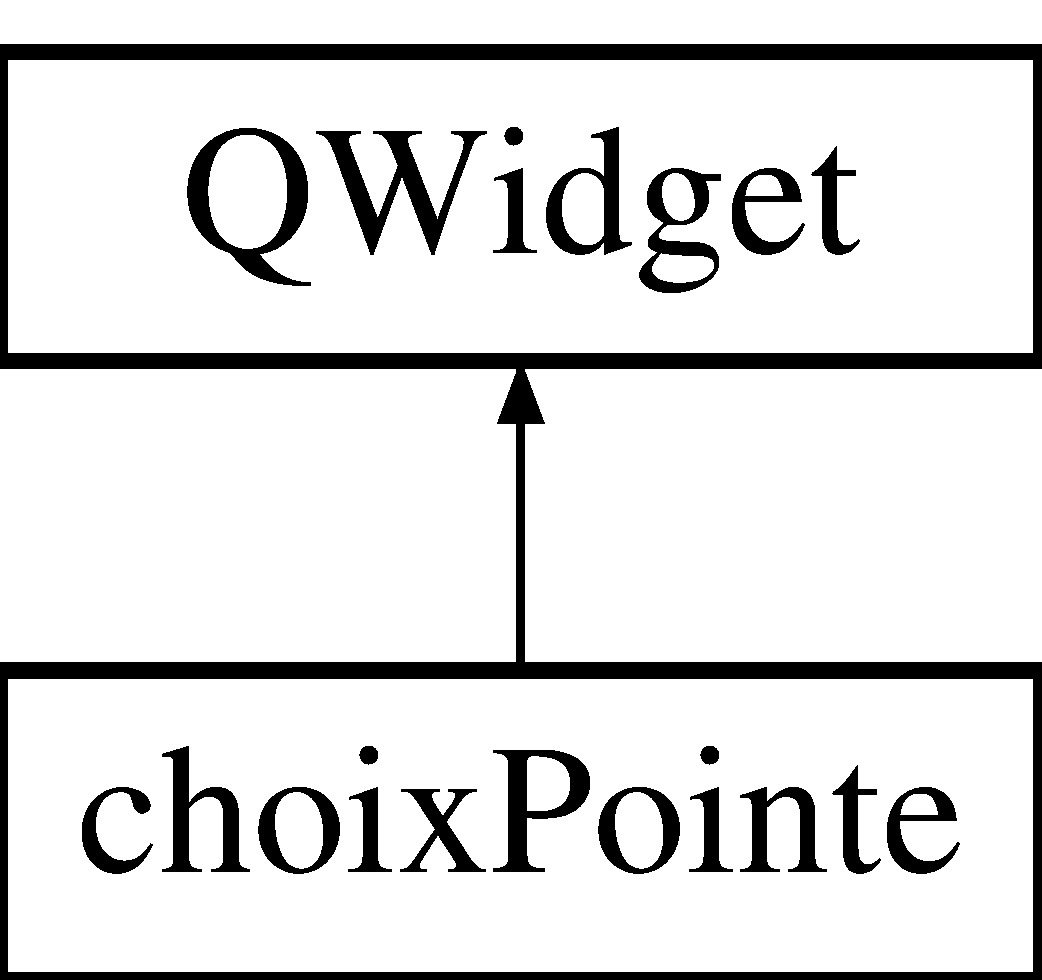
\includegraphics[height=2.000000cm]{classchoix_pointe}
\end{center}
\end{figure}
\subsection*{Public Slots}
\begin{DoxyCompactItemize}
\item 
\hypertarget{classchoix_pointe_ac8ccad58270933a4950d5c6e2cc74168}{void {\bfseries send\-Dad} ()}\label{classchoix_pointe_ac8ccad58270933a4950d5c6e2cc74168}

\end{DoxyCompactItemize}
\subsection*{Signals}
\begin{DoxyCompactItemize}
\item 
\hypertarget{classchoix_pointe_a586763c92b709e2e5d0b27c412e62ec2}{void {\bfseries add} (int cible, int vocab)}\label{classchoix_pointe_a586763c92b709e2e5d0b27c412e62ec2}

\end{DoxyCompactItemize}
\subsection*{Public Member Functions}
\begin{DoxyCompactItemize}
\item 
\hypertarget{classchoix_pointe_adb585f204f3b658650d3a4b42d871e04}{{\bfseries choix\-Pointe} (Q\-Widget $\ast$parent=0)}\label{classchoix_pointe_adb585f204f3b658650d3a4b42d871e04}

\item 
\hypertarget{classchoix_pointe_a8c91319071281be73b5d762dfa985bbd}{void {\bfseries reset\-Affichage} (\hyperlink{class_automate}{Automate})}\label{classchoix_pointe_a8c91319071281be73b5d762dfa985bbd}

\end{DoxyCompactItemize}
\subsection*{Protected Member Functions}
\begin{DoxyCompactItemize}
\item 
\hypertarget{classchoix_pointe_a7becbc30c1a5f930c98336623595d181}{void {\bfseries change\-Event} (Q\-Event $\ast$e)}\label{classchoix_pointe_a7becbc30c1a5f930c98336623595d181}

\end{DoxyCompactItemize}


The documentation for this class was generated from the following files\-:\begin{DoxyCompactItemize}
\item 
/home/aaiiighht/\-Bureau/projet\-T\-L/automate-\/project/choixpointe.\-h\item 
/home/aaiiighht/\-Bureau/projet\-T\-L/automate-\/project/choixpointe.\-cpp\item 
/home/aaiiighht/\-Bureau/projet\-T\-L/automate-\/project/moc\-\_\-choixpointe.\-cpp\end{DoxyCompactItemize}

\hypertarget{class_ui_1_1choix_pointe}{\section{Ui\-:\-:choix\-Pointe Class Reference}
\label{class_ui_1_1choix_pointe}\index{Ui\-::choix\-Pointe@{Ui\-::choix\-Pointe}}
}
Inheritance diagram for Ui\-:\-:choix\-Pointe\-:\begin{figure}[H]
\begin{center}
\leavevmode
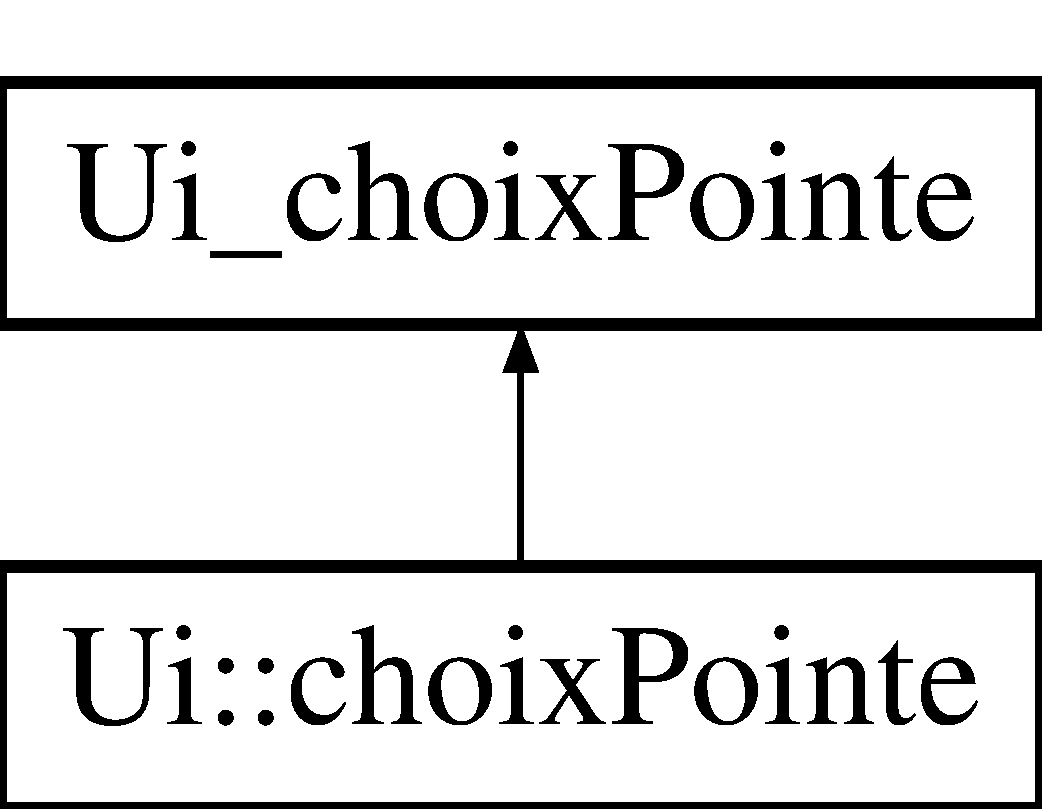
\includegraphics[height=2.000000cm]{class_ui_1_1choix_pointe}
\end{center}
\end{figure}
\subsection*{Additional Inherited Members}


The documentation for this class was generated from the following file\-:\begin{DoxyCompactItemize}
\item 
/home/aaiiighht/\-Bureau/projet\-T\-L/automate-\/project/ui\-\_\-choixpointe.\-h\end{DoxyCompactItemize}

\hypertarget{class_ui_1_1_create_automate}{\section{Ui\-:\-:Create\-Automate Class Reference}
\label{class_ui_1_1_create_automate}\index{Ui\-::\-Create\-Automate@{Ui\-::\-Create\-Automate}}
}


Inheritance diagram for Ui\-:\-:Create\-Automate\-:
\nopagebreak
\begin{figure}[H]
\begin{center}
\leavevmode
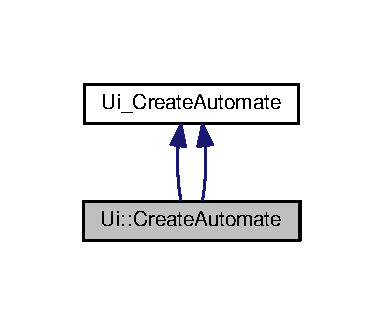
\includegraphics[width=184pt]{class_ui_1_1_create_automate__inherit__graph}
\end{center}
\end{figure}


Collaboration diagram for Ui\-:\-:Create\-Automate\-:
\nopagebreak
\begin{figure}[H]
\begin{center}
\leavevmode
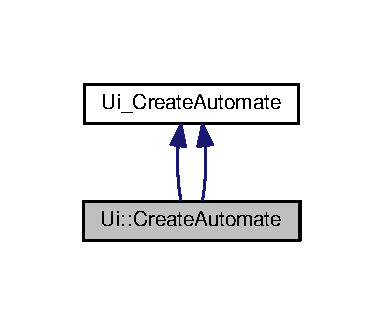
\includegraphics[width=184pt]{class_ui_1_1_create_automate__coll__graph}
\end{center}
\end{figure}
\subsection*{Additional Inherited Members}


The documentation for this class was generated from the following file\-:\begin{DoxyCompactItemize}
\item 
/home/aaiiighht/\-Bureau/smartgit/bin/projet\-T\-L/automate-\/project/release/ui\-\_\-createautomate.\-h\end{DoxyCompactItemize}

\hypertarget{class_create_automate}{\section{Create\-Automate Class Reference}
\label{class_create_automate}\index{Create\-Automate@{Create\-Automate}}
}
Inheritance diagram for Create\-Automate\-:\begin{figure}[H]
\begin{center}
\leavevmode
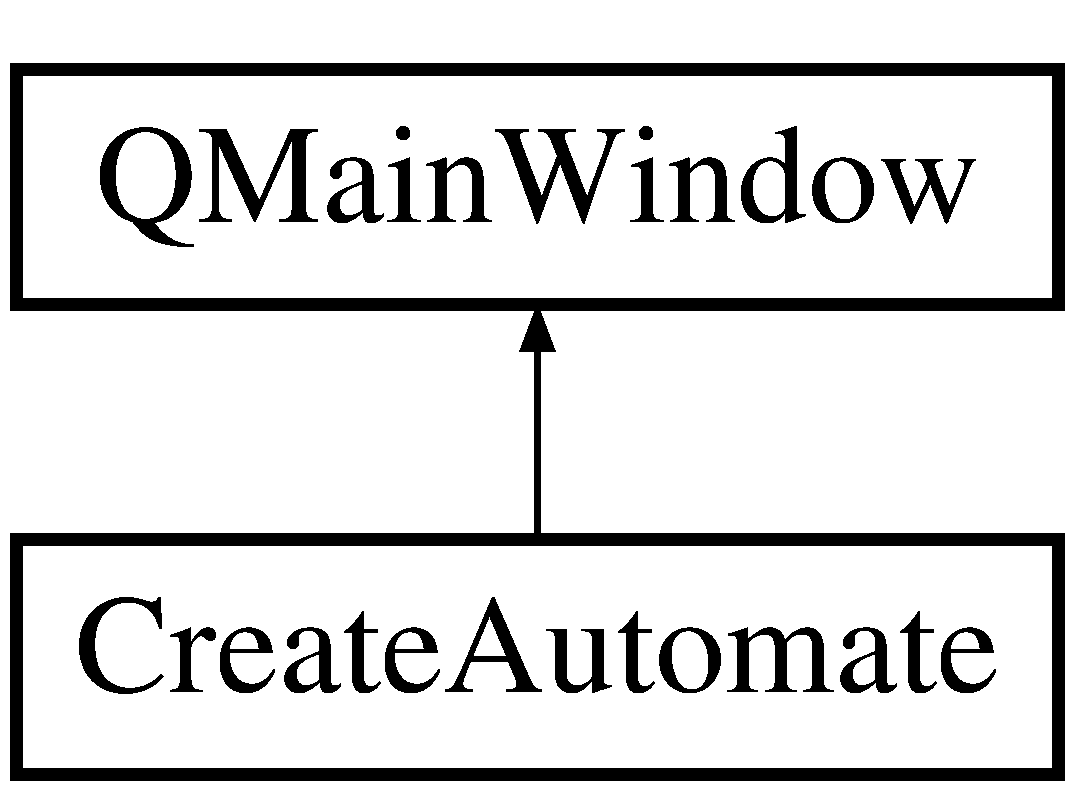
\includegraphics[height=2.000000cm]{class_create_automate}
\end{center}
\end{figure}
\subsection*{Public Slots}
\begin{DoxyCompactItemize}
\item 
void \hyperlink{class_create_automate_aa0b73cfa67f2921a14d69c8d7345ae53}{ajout\-Etat} (bool ini=false, bool fina=false)
\begin{DoxyCompactList}\small\item\em Ajoute un état à la fenetre. \end{DoxyCompactList}\item 
\hypertarget{class_create_automate_a66a9d64abf7e1ad5e4ac7611491d32e5}{void \hyperlink{class_create_automate_a66a9d64abf7e1ad5e4ac7611491d32e5}{afficher\-Automate} ()}\label{class_create_automate_a66a9d64abf7e1ad5e4ac7611491d32e5}

\begin{DoxyCompactList}\small\item\em Affiche un automate en grand. \end{DoxyCompactList}\item 
void \hyperlink{class_create_automate_a5477eeb6bd6dd910d74aa4e7ee608a54}{display\-Right} (int to\-Display)
\begin{DoxyCompactList}\small\item\em Affiche l'etat right spécifié \end{DoxyCompactList}\item 
void \hyperlink{class_create_automate_aa9abcb9364d0fc6fd01193cc3cdec08c}{supprime\-Etat} (int cible)
\begin{DoxyCompactList}\small\item\em Supprime un état et réactualise l'affichage. \end{DoxyCompactList}\item 
\hypertarget{class_create_automate_afda9720982becab25e51355c0e1e5d89}{void \hyperlink{class_create_automate_afda9720982becab25e51355c0e1e5d89}{refresh\-All} ()}\label{class_create_automate_afda9720982becab25e51355c0e1e5d89}

\begin{DoxyCompactList}\small\item\em Réactualise tout l'affichage. \end{DoxyCompactList}\item 
\hypertarget{class_create_automate_a257c028c9d44547b9e3940b9260a1260}{void \hyperlink{class_create_automate_a257c028c9d44547b9e3940b9260a1260}{sauvegarder} ()}\label{class_create_automate_a257c028c9d44547b9e3940b9260a1260}

\begin{DoxyCompactList}\small\item\em Sauvegarder l'automate créé \end{DoxyCompactList}\item 
void \hyperlink{class_create_automate_a107306a68c03913c6d971c4fbd16efa5}{change\-State} (int \hyperlink{classetat}{etat}, bool ini, bool final)
\begin{DoxyCompactList}\small\item\em Modifie un état. \end{DoxyCompactList}\end{DoxyCompactItemize}
\subsection*{Public Member Functions}
\begin{DoxyCompactItemize}
\item 
\hyperlink{class_create_automate_a564b1212466be9837975faf60f115862}{Create\-Automate} (Q\-Widget $\ast$parent=0)
\begin{DoxyCompactList}\small\item\em Constructeur. \end{DoxyCompactList}\item 
\hypertarget{class_create_automate_a936c5cf4d629a68ede5779b656061428}{\hyperlink{class_create_automate_a936c5cf4d629a68ede5779b656061428}{$\sim$\-Create\-Automate} ()}\label{class_create_automate_a936c5cf4d629a68ede5779b656061428}

\begin{DoxyCompactList}\small\item\em Destructeur. \end{DoxyCompactList}\item 
\hypertarget{class_create_automate_a13c0f6c01986d1ef1173c84e7ff01768}{void \hyperlink{class_create_automate_a13c0f6c01986d1ef1173c84e7ff01768}{reset\-All\-List\-Choix} ()}\label{class_create_automate_a13c0f6c01986d1ef1173c84e7ff01768}

\begin{DoxyCompactList}\small\item\em Remet à jour la liste des états de droite. \end{DoxyCompactList}\item 
\hypertarget{class_create_automate_ae3ab55bac630576c180865589a10c765}{void \hyperlink{class_create_automate_ae3ab55bac630576c180865589a10c765}{display\-Automate} ()}\label{class_create_automate_ae3ab55bac630576c180865589a10c765}

\begin{DoxyCompactList}\small\item\em Réactualise l'affichage de l'automate dans ma\-Vue. \end{DoxyCompactList}\end{DoxyCompactItemize}
\subsection*{Public Attributes}
\begin{DoxyCompactItemize}
\item 
\hyperlink{class_automate}{Automate} \hyperlink{class_create_automate_a00809917dbe83828485789bf25725964}{a}
\item 
Q\-Svg\-Widget $\ast$ \hyperlink{class_create_automate_a67da1a6995daa455a00771c099358a89}{ma\-Vue}
\item 
\hypertarget{class_create_automate_a599db4453047381fcd0d48dfb185da82}{int {\bfseries actuel}}\label{class_create_automate_a599db4453047381fcd0d48dfb185da82}

\item 
vector$<$ \hyperlink{classetat_left}{etat\-Left} $\ast$ $>$ \hyperlink{class_create_automate_a368e5fd06e6bafb6a297cb7d32d90655}{left}
\item 
vector$<$ \hyperlink{classetat_right}{etat\-Right} $\ast$ $>$ \hyperlink{class_create_automate_a8471078665ab7f4daf858c81f35496ac}{right}
\end{DoxyCompactItemize}
\subsection*{Protected Member Functions}
\begin{DoxyCompactItemize}
\item 
\hypertarget{class_create_automate_acae0d3eabf60d2ae32f75ad11aa59be6}{void {\bfseries change\-Event} (Q\-Event $\ast$e)}\label{class_create_automate_acae0d3eabf60d2ae32f75ad11aa59be6}

\item 
\hypertarget{class_create_automate_aad4103629c0487ca511f43502c290be0}{void \hyperlink{class_create_automate_aad4103629c0487ca511f43502c290be0}{adjust} ()}\label{class_create_automate_aad4103629c0487ca511f43502c290be0}

\begin{DoxyCompactList}\small\item\em Ajuste l'affichage. \end{DoxyCompactList}\end{DoxyCompactItemize}


\subsection{Constructor \& Destructor Documentation}
\hypertarget{class_create_automate_a564b1212466be9837975faf60f115862}{\index{Create\-Automate@{Create\-Automate}!Create\-Automate@{Create\-Automate}}
\index{Create\-Automate@{Create\-Automate}!CreateAutomate@{Create\-Automate}}
\subsubsection[{Create\-Automate}]{\setlength{\rightskip}{0pt plus 5cm}Create\-Automate\-::\-Create\-Automate (
\begin{DoxyParamCaption}
\item[{Q\-Widget $\ast$}]{parent = {\ttfamily 0}}
\end{DoxyParamCaption}
)}}\label{class_create_automate_a564b1212466be9837975faf60f115862}


Constructeur. 

Instancie cette partie de la fenêtre. 

\subsection{Member Function Documentation}
\hypertarget{class_create_automate_aa0b73cfa67f2921a14d69c8d7345ae53}{\index{Create\-Automate@{Create\-Automate}!ajout\-Etat@{ajout\-Etat}}
\index{ajout\-Etat@{ajout\-Etat}!CreateAutomate@{Create\-Automate}}
\subsubsection[{ajout\-Etat}]{\setlength{\rightskip}{0pt plus 5cm}void Create\-Automate\-::ajout\-Etat (
\begin{DoxyParamCaption}
\item[{bool}]{ini = {\ttfamily false}, }
\item[{bool}]{fina = {\ttfamily false}}
\end{DoxyParamCaption}
)\hspace{0.3cm}{\ttfamily [slot]}}}\label{class_create_automate_aa0b73cfa67f2921a14d69c8d7345ae53}


Ajoute un état à la fenetre. 

Construit un etat left et right associé à ce nouvel état.


\begin{DoxyParams}{Parameters}
{\em ini} & \-: true si l'état est initial \\
\hline
{\em fina} & \-: true si l'état est final \\
\hline
\end{DoxyParams}
\hypertarget{class_create_automate_a107306a68c03913c6d971c4fbd16efa5}{\index{Create\-Automate@{Create\-Automate}!change\-State@{change\-State}}
\index{change\-State@{change\-State}!CreateAutomate@{Create\-Automate}}
\subsubsection[{change\-State}]{\setlength{\rightskip}{0pt plus 5cm}void Create\-Automate\-::change\-State (
\begin{DoxyParamCaption}
\item[{int}]{etat, }
\item[{bool}]{ini, }
\item[{bool}]{final}
\end{DoxyParamCaption}
)\hspace{0.3cm}{\ttfamily [slot]}}}\label{class_create_automate_a107306a68c03913c6d971c4fbd16efa5}


Modifie un état. 


\begin{DoxyParams}{Parameters}
{\em etat} & \-: l'état à modifier \\
\hline
{\em ini} & \-: true si l'état est initial \\
\hline
{\em final} & \-: true si l'état est final \\
\hline
\end{DoxyParams}
\hypertarget{class_create_automate_a5477eeb6bd6dd910d74aa4e7ee608a54}{\index{Create\-Automate@{Create\-Automate}!display\-Right@{display\-Right}}
\index{display\-Right@{display\-Right}!CreateAutomate@{Create\-Automate}}
\subsubsection[{display\-Right}]{\setlength{\rightskip}{0pt plus 5cm}void Create\-Automate\-::display\-Right (
\begin{DoxyParamCaption}
\item[{int}]{to\-Display}
\end{DoxyParamCaption}
)\hspace{0.3cm}{\ttfamily [slot]}}}\label{class_create_automate_a5477eeb6bd6dd910d74aa4e7ee608a54}


Affiche l'etat right spécifié 


\begin{DoxyParams}{Parameters}
{\em to\-Display} & \-: l'état à afficher \\
\hline
\end{DoxyParams}
\hypertarget{class_create_automate_aa9abcb9364d0fc6fd01193cc3cdec08c}{\index{Create\-Automate@{Create\-Automate}!supprime\-Etat@{supprime\-Etat}}
\index{supprime\-Etat@{supprime\-Etat}!CreateAutomate@{Create\-Automate}}
\subsubsection[{supprime\-Etat}]{\setlength{\rightskip}{0pt plus 5cm}void Create\-Automate\-::supprime\-Etat (
\begin{DoxyParamCaption}
\item[{int}]{cible}
\end{DoxyParamCaption}
)\hspace{0.3cm}{\ttfamily [slot]}}}\label{class_create_automate_aa9abcb9364d0fc6fd01193cc3cdec08c}


Supprime un état et réactualise l'affichage. 


\begin{DoxyParams}{Parameters}
{\em cible} & \-: l'état à supprimer \\
\hline
\end{DoxyParams}


\subsection{Member Data Documentation}
\hypertarget{class_create_automate_a00809917dbe83828485789bf25725964}{\index{Create\-Automate@{Create\-Automate}!a@{a}}
\index{a@{a}!CreateAutomate@{Create\-Automate}}
\subsubsection[{a}]{\setlength{\rightskip}{0pt plus 5cm}{\bf Automate} Create\-Automate\-::a}}\label{class_create_automate_a00809917dbe83828485789bf25725964}
L'automate en train d'être construit \hypertarget{class_create_automate_a368e5fd06e6bafb6a297cb7d32d90655}{\index{Create\-Automate@{Create\-Automate}!left@{left}}
\index{left@{left}!CreateAutomate@{Create\-Automate}}
\subsubsection[{left}]{\setlength{\rightskip}{0pt plus 5cm}vector$<${\bf etat\-Left}$\ast$$>$ Create\-Automate\-::left}}\label{class_create_automate_a368e5fd06e6bafb6a297cb7d32d90655}
Vecteur représentant les états déjà construits \hypertarget{class_create_automate_a67da1a6995daa455a00771c099358a89}{\index{Create\-Automate@{Create\-Automate}!ma\-Vue@{ma\-Vue}}
\index{ma\-Vue@{ma\-Vue}!CreateAutomate@{Create\-Automate}}
\subsubsection[{ma\-Vue}]{\setlength{\rightskip}{0pt plus 5cm}Q\-Svg\-Widget$\ast$ Create\-Automate\-::ma\-Vue}}\label{class_create_automate_a67da1a6995daa455a00771c099358a89}
Partie inférieure droite de la fenetre, où l'automate est affiché \hypertarget{class_create_automate_a8471078665ab7f4daf858c81f35496ac}{\index{Create\-Automate@{Create\-Automate}!right@{right}}
\index{right@{right}!CreateAutomate@{Create\-Automate}}
\subsubsection[{right}]{\setlength{\rightskip}{0pt plus 5cm}vector$<${\bf etat\-Right}$\ast$$>$ Create\-Automate\-::right}}\label{class_create_automate_a8471078665ab7f4daf858c81f35496ac}
Vecteur dont chaque élément représente une transition a modifié éventuellement pour un état 

The documentation for this class was generated from the following files\-:\begin{DoxyCompactItemize}
\item 
/home/aaiiighht/\-Bureau/projet\-T\-L/automate-\/project/\hyperlink{createautomate_8h}{createautomate.\-h}\item 
/home/aaiiighht/\-Bureau/projet\-T\-L/automate-\/project/createautomate.\-cpp\end{DoxyCompactItemize}

\hypertarget{classetat}{\section{etat Class Reference}
\label{classetat}\index{etat@{etat}}
}
\subsection*{Public Member Functions}
\begin{DoxyCompactItemize}
\item 
\hypertarget{classetat_a65b2ac734cc1af21fb1aea8fb873d4c9}{{\bfseries etat} (int, bool ini=false, bool fina=false)}\label{classetat_a65b2ac734cc1af21fb1aea8fb873d4c9}

\item 
\hypertarget{classetat_af42b35ca878600e1877052978a11303f}{{\bfseries etat} (const \hyperlink{classetat}{etat} \&e)}\label{classetat_af42b35ca878600e1877052978a11303f}

\item 
\hypertarget{classetat_a0eeba3eaa0ce8633957d309f04f07995}{int {\bfseries get\-Number} ()}\label{classetat_a0eeba3eaa0ce8633957d309f04f07995}

\item 
\hypertarget{classetat_ab771b2354397b5b4d3ead9a62668d44f}{void {\bfseries set\-Number} (int)}\label{classetat_ab771b2354397b5b4d3ead9a62668d44f}

\item 
\hypertarget{classetat_a89188d6ea23ce287c3f3afda46fa2858}{bool {\bfseries is\-Final} ()}\label{classetat_a89188d6ea23ce287c3f3afda46fa2858}

\item 
\hypertarget{classetat_ae4daff4d04de194b976ad489eeceb07d}{void {\bfseries set\-Final} (bool)}\label{classetat_ae4daff4d04de194b976ad489eeceb07d}

\item 
\hypertarget{classetat_a6993bd53bfd754392515e4ef5772fcdc}{bool {\bfseries is\-Initial} ()}\label{classetat_a6993bd53bfd754392515e4ef5772fcdc}

\item 
\hypertarget{classetat_a2c3e2a7b1bfda47c137aa3f6b563e369}{void {\bfseries set\-Initial} (bool)}\label{classetat_a2c3e2a7b1bfda47c137aa3f6b563e369}

\item 
\hypertarget{classetat_a3d94a2b3e6f60c9475b142e28ea495b4}{void {\bfseries ajout\-Transition} (\hyperlink{classetat}{etat}, int)}\label{classetat_a3d94a2b3e6f60c9475b142e28ea495b4}

\item 
\hypertarget{classetat_a87328ea8752e2396ac15f2465f2ff315}{void {\bfseries supprime\-Transition} (\hyperlink{classetat}{etat}, int)}\label{classetat_a87328ea8752e2396ac15f2465f2ff315}

\item 
\hypertarget{classetat_a8e195072b1adca99801b6a4a432eb9f8}{void {\bfseries rename\-Transition} (\hyperlink{classetat}{etat}, int)}\label{classetat_a8e195072b1adca99801b6a4a432eb9f8}

\item 
\hypertarget{classetat_acc168f9b970e301d65e72cf1f4ee9062}{multimap$<$ int, \hyperlink{classetat}{etat} $>$ {\bfseries get\-Transitions} ()}\label{classetat_acc168f9b970e301d65e72cf1f4ee9062}

\item 
\hypertarget{classetat_a0a1950caa3737139ea5dc29c600e842d}{bool {\bfseries operator==} (\hyperlink{classetat}{etat} \&) const }\label{classetat_a0a1950caa3737139ea5dc29c600e842d}

\item 
\hypertarget{classetat_ab6f5ff8cf0dadb8b9be06095ae3b2c49}{bool {\bfseries operator!=} (\hyperlink{classetat}{etat} \&) const }\label{classetat_ab6f5ff8cf0dadb8b9be06095ae3b2c49}

\item 
\hypertarget{classetat_acab203fc095b3974136c4f73895df9a6}{bool {\bfseries find\-\_\-transition} (int etiq, \hyperlink{classetat}{etat} e)}\label{classetat_acab203fc095b3974136c4f73895df9a6}

\item 
\hypertarget{classetat_a381028a7a37e890734c1cc4afe05bd55}{bool {\bfseries est\-Dans\-List} (list$<$ \hyperlink{classetat}{etat} $>$ liste)}\label{classetat_a381028a7a37e890734c1cc4afe05bd55}

\item 
\hypertarget{classetat_a65ef0b41b54bbf36b5dab8071822171d}{void {\bfseries set\-Name} (string)}\label{classetat_a65ef0b41b54bbf36b5dab8071822171d}

\item 
\hypertarget{classetat_a938d2165beabfb6de3ad16e2a15b05c5}{string {\bfseries get\-Name} ()}\label{classetat_a938d2165beabfb6de3ad16e2a15b05c5}

\item 
\hypertarget{classetat_a37ee0f6502f471dd3566733f8a1bc8fe}{string {\bfseries get\-Name\-F} ()}\label{classetat_a37ee0f6502f471dd3566733f8a1bc8fe}

\item 
\hypertarget{classetat_a87882f3b4b4e3bae6b7a22008241d836}{void {\bfseries set\-Name} (list$<$ \hyperlink{classetat}{etat} $>$ l)}\label{classetat_a87882f3b4b4e3bae6b7a22008241d836}

\end{DoxyCompactItemize}
\subsection*{Public Attributes}
\begin{DoxyCompactItemize}
\item 
\hypertarget{classetat_a155cdfece54b9e8f4a633249ee037595}{int {\bfseries numero}}\label{classetat_a155cdfece54b9e8f4a633249ee037595}

\end{DoxyCompactItemize}


The documentation for this class was generated from the following files\-:\begin{DoxyCompactItemize}
\item 
/home/aaiiighht/\-Bureau/smartgit/bin/projet\-T\-L/automate-\/project/etat.\-h\item 
/home/aaiiighht/\-Bureau/smartgit/bin/projet\-T\-L/automate-\/project/etat.\-cpp\end{DoxyCompactItemize}

\hypertarget{classetat_left}{\section{etat\-Left Class Reference}
\label{classetat_left}\index{etat\-Left@{etat\-Left}}
}
Inheritance diagram for etat\-Left\-:\begin{figure}[H]
\begin{center}
\leavevmode
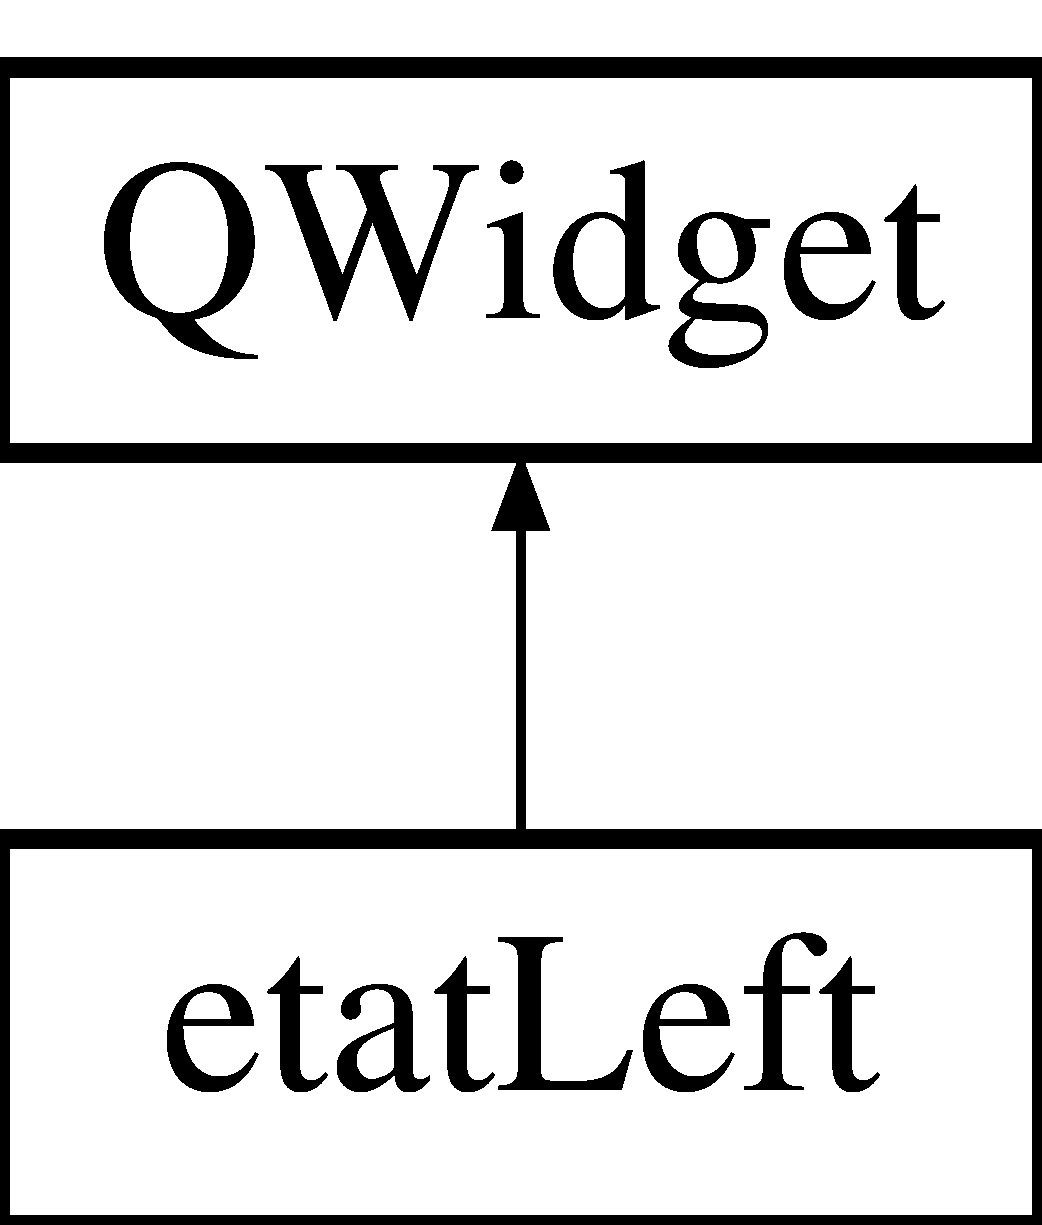
\includegraphics[height=2.000000cm]{classetat_left}
\end{center}
\end{figure}
\subsection*{Public Slots}
\begin{DoxyCompactItemize}
\item 
\hypertarget{classetat_left_a39c9a7992253a787aeaa9a2b2be5a806}{void {\bfseries send\-Dad} ()}\label{classetat_left_a39c9a7992253a787aeaa9a2b2be5a806}

\item 
\hypertarget{classetat_left_a541d2de7f5227a558e6753f53c6b7ae6}{void {\bfseries ask\-For\-Supress} ()}\label{classetat_left_a541d2de7f5227a558e6753f53c6b7ae6}

\end{DoxyCompactItemize}
\subsection*{Signals}
\begin{DoxyCompactItemize}
\item 
\hypertarget{classetat_left_a9c96e4ffbba54cfc6c281e4ab023b4e6}{void {\bfseries selected} (int me)}\label{classetat_left_a9c96e4ffbba54cfc6c281e4ab023b4e6}

\item 
\hypertarget{classetat_left_a8d4e53e9e84d7865f1f95f404cb55132}{void {\bfseries supress} (int)}\label{classetat_left_a8d4e53e9e84d7865f1f95f404cb55132}

\end{DoxyCompactItemize}
\subsection*{Public Member Functions}
\begin{DoxyCompactItemize}
\item 
\hypertarget{classetat_left_ac7e09685da20850a612f710d3db145f7}{{\bfseries etat\-Left} (int, Q\-Widget $\ast$parent=0)}\label{classetat_left_ac7e09685da20850a612f710d3db145f7}

\end{DoxyCompactItemize}
\subsection*{Protected Member Functions}
\begin{DoxyCompactItemize}
\item 
\hypertarget{classetat_left_a3509079b87d2584825e12adddcfb1a32}{void {\bfseries change\-Event} (Q\-Event $\ast$e)}\label{classetat_left_a3509079b87d2584825e12adddcfb1a32}

\end{DoxyCompactItemize}
\subsection*{Protected Attributes}
\begin{DoxyCompactItemize}
\item 
\hypertarget{classetat_left_acf1c86368edc9def78782bf5db7aa651}{int {\bfseries numero}}\label{classetat_left_acf1c86368edc9def78782bf5db7aa651}

\end{DoxyCompactItemize}


The documentation for this class was generated from the following files\-:\begin{DoxyCompactItemize}
\item 
/home/aaiiighht/\-Bureau/projet\-T\-L/automate-\/project/etatleft.\-h\item 
/home/aaiiighht/\-Bureau/projet\-T\-L/automate-\/project/etatleft.\-cpp\item 
/home/aaiiighht/\-Bureau/projet\-T\-L/automate-\/project/moc\-\_\-etatleft.\-cpp\end{DoxyCompactItemize}

\hypertarget{class_ui_1_1etat_left}{\section{Ui\-:\-:etat\-Left Class Reference}
\label{class_ui_1_1etat_left}\index{Ui\-::etat\-Left@{Ui\-::etat\-Left}}
}
Inheritance diagram for Ui\-:\-:etat\-Left\-:\begin{figure}[H]
\begin{center}
\leavevmode
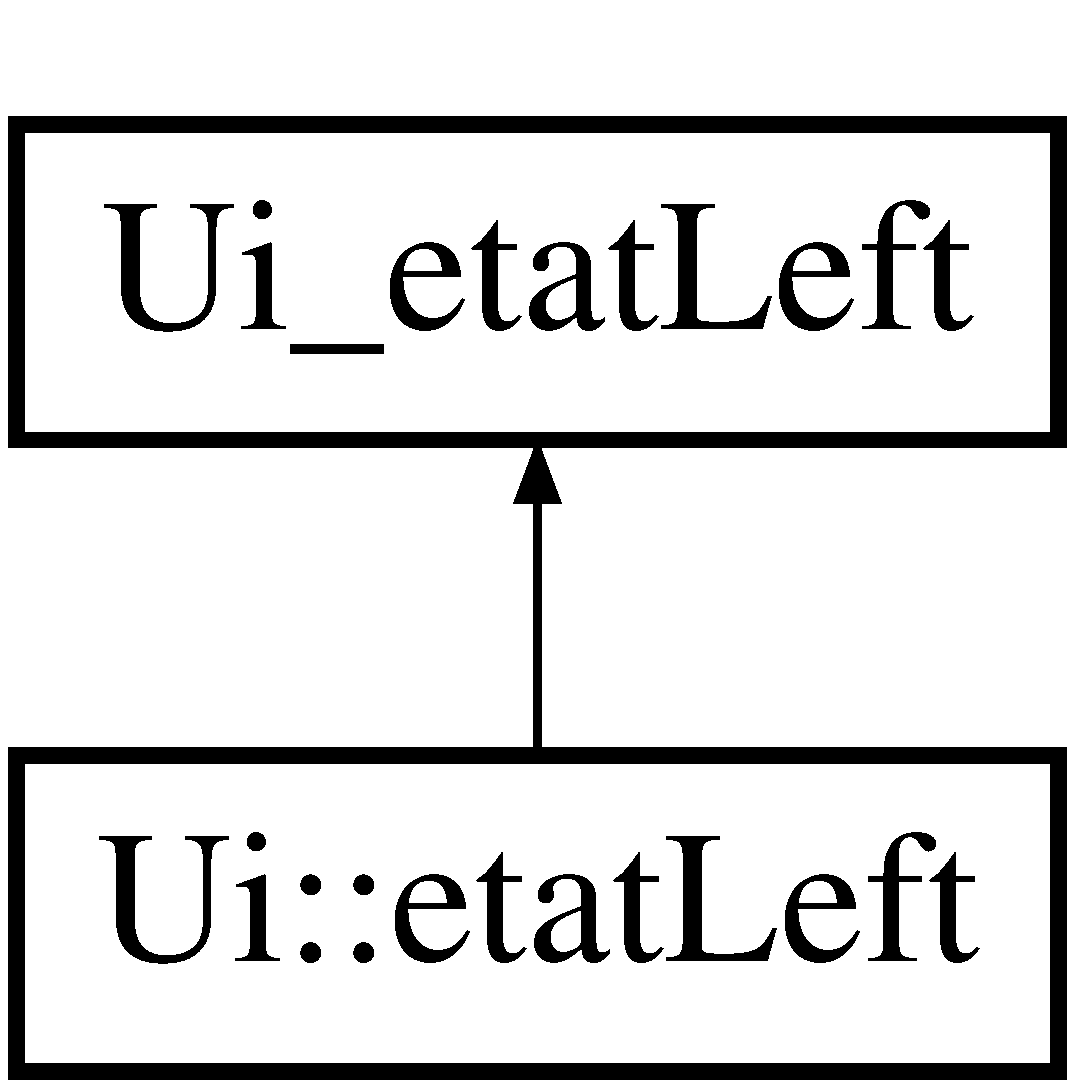
\includegraphics[height=2.000000cm]{class_ui_1_1etat_left}
\end{center}
\end{figure}
\subsection*{Additional Inherited Members}


The documentation for this class was generated from the following file\-:\begin{DoxyCompactItemize}
\item 
/home/aaiiighht/\-Bureau/projet\-T\-L/automate-\/project/ui\-\_\-etatleft.\-h\end{DoxyCompactItemize}

\hypertarget{class_ui_1_1etat_right}{\section{Ui\-:\-:etat\-Right Class Reference}
\label{class_ui_1_1etat_right}\index{Ui\-::etat\-Right@{Ui\-::etat\-Right}}
}
Inheritance diagram for Ui\-:\-:etat\-Right\-:\begin{figure}[H]
\begin{center}
\leavevmode
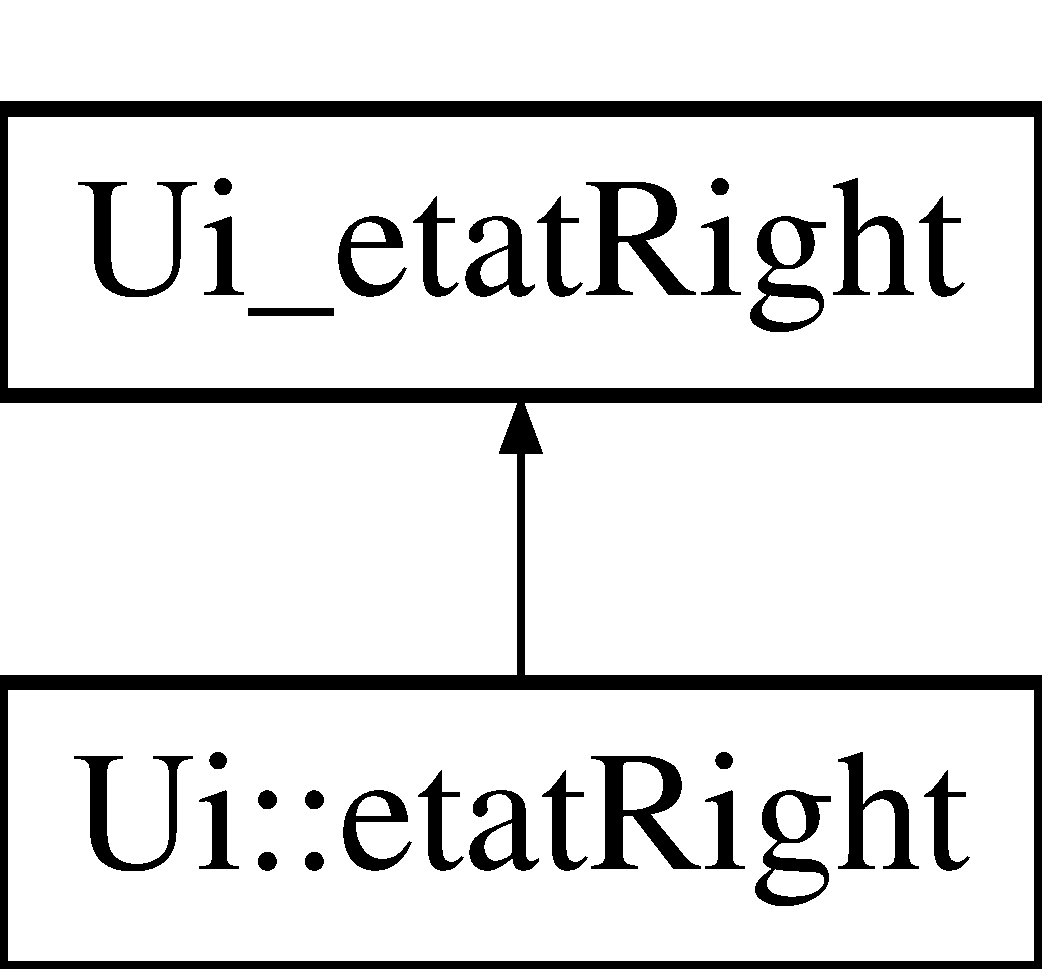
\includegraphics[height=2.000000cm]{class_ui_1_1etat_right}
\end{center}
\end{figure}
\subsection*{Additional Inherited Members}


The documentation for this class was generated from the following file\-:\begin{DoxyCompactItemize}
\item 
/home/aaiiighht/\-Bureau/projet\-T\-L/automate-\/project/ui\-\_\-etatright.\-h\end{DoxyCompactItemize}

\hypertarget{classetat_right}{\section{etat\-Right Class Reference}
\label{classetat_right}\index{etat\-Right@{etat\-Right}}
}
Inheritance diagram for etat\-Right\-:\begin{figure}[H]
\begin{center}
\leavevmode
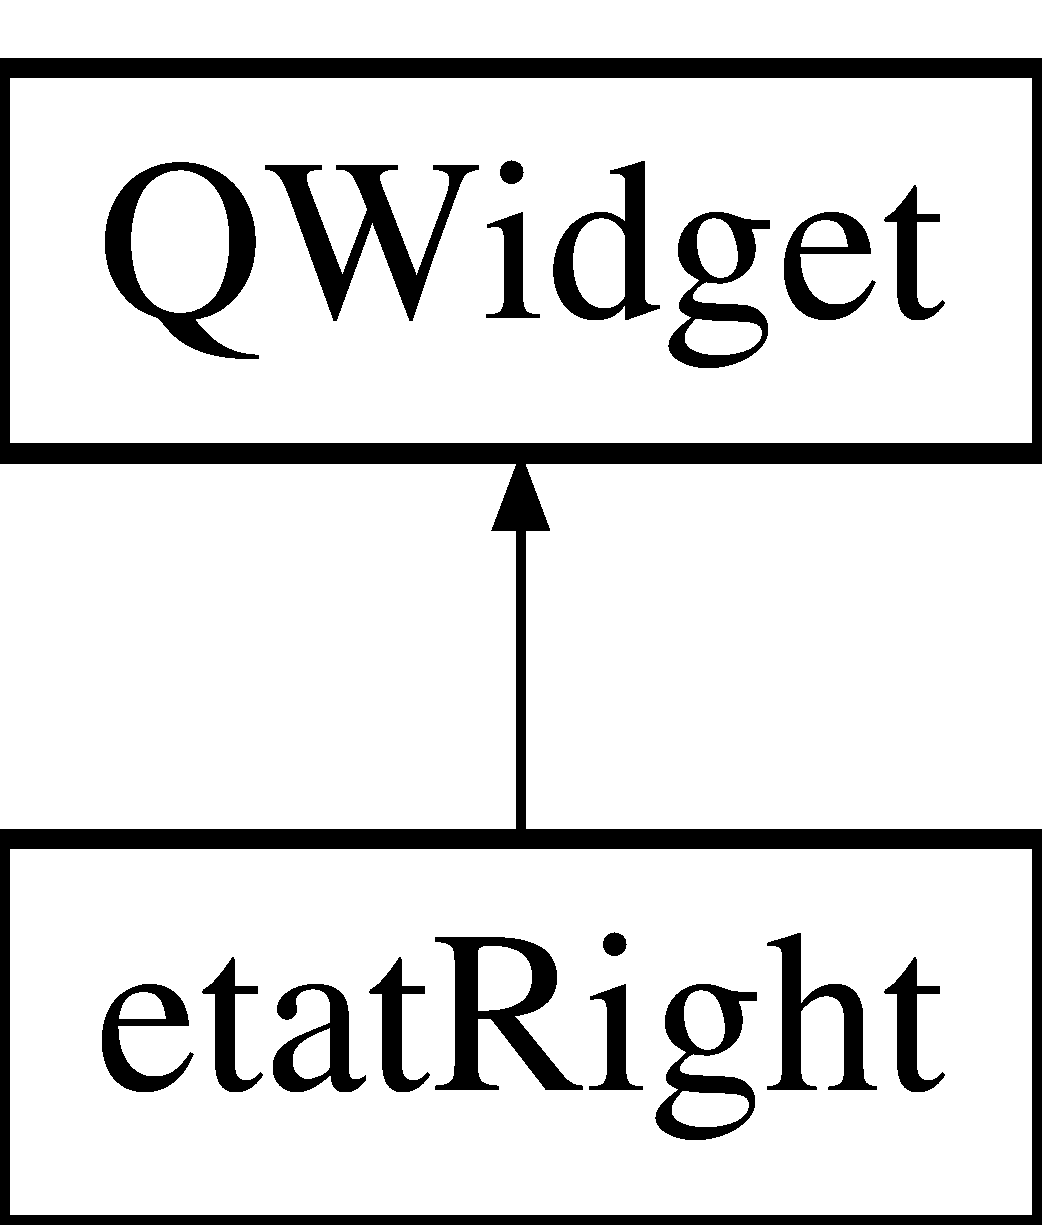
\includegraphics[height=2.000000cm]{classetat_right}
\end{center}
\end{figure}
\subsection*{Public Slots}
\begin{DoxyCompactItemize}
\item 
void \hyperlink{classetat_right_a384a6718c6a76d7ad6c49ce8942e0f93}{add\-Transition} (int to, int vocab)
\begin{DoxyCompactList}\small\item\em Ajout d'une transition. \end{DoxyCompactList}\item 
void \hyperlink{classetat_right_a0ea39c8d918126244c9ecbf11b46a0ae}{erase\-Transition} (int to, int vocab)
\begin{DoxyCompactList}\small\item\em Suppresion d'une transition. \end{DoxyCompactList}\item 
\hypertarget{classetat_right_ac15456fc1dacf084b9bcbae7d6699627}{void {\bfseries etat\-Change} ()}\label{classetat_right_ac15456fc1dacf084b9bcbae7d6699627}

\end{DoxyCompactItemize}
\subsection*{Signals}
\begin{DoxyCompactItemize}
\item 
\hypertarget{classetat_right_ac7e6e4cff96fe796b6dcf1c4fca96e48}{void {\bfseries refresh\-Needed} (int)}\label{classetat_right_ac7e6e4cff96fe796b6dcf1c4fca96e48}

\item 
\hypertarget{classetat_right_a4ee395991e158ac64118b802d23b0962}{void {\bfseries etat\-Changes} (int, bool, bool)}\label{classetat_right_a4ee395991e158ac64118b802d23b0962}

\end{DoxyCompactItemize}
\subsection*{Public Member Functions}
\begin{DoxyCompactItemize}
\item 
\hyperlink{classetat_right_a9f171541e1762e55588f569a6c168dd3}{etat\-Right} (\hyperlink{class_automate}{Automate} $\ast$\hyperlink{classetat_right_aa6d344e0bd745915bfb4ea0e767f0bc0}{a}, int, Q\-Widget $\ast$parent=0)
\begin{DoxyCompactList}\small\item\em Constructeur. \end{DoxyCompactList}\item 
\hypertarget{classetat_right_a3e242d2baf785c43643f0bf9d8dec58f}{\hyperlink{classetat_right_a3e242d2baf785c43643f0bf9d8dec58f}{$\sim$etat\-Right} ()}\label{classetat_right_a3e242d2baf785c43643f0bf9d8dec58f}

\begin{DoxyCompactList}\small\item\em Destructeur. \end{DoxyCompactList}\item 
\hypertarget{classetat_right_a6631d8b4878cdaa7c8443c24825fd791}{void \hyperlink{classetat_right_a6631d8b4878cdaa7c8443c24825fd791}{remplir\-List\-Choix} ()}\label{classetat_right_a6631d8b4878cdaa7c8443c24825fd791}

\begin{DoxyCompactList}\small\item\em Remet à jour la liste dans \hyperlink{classchoix_pointe}{choix\-Pointe} permettant de choisir l'etat cible de la transition. \end{DoxyCompactList}\item 
\hypertarget{classetat_right_a9bd49810066fc43059d2adf138784fd6}{void {\bfseries add\-Visual\-Transition} (int, int)}\label{classetat_right_a9bd49810066fc43059d2adf138784fd6}

\item 
\hypertarget{classetat_right_a181683fbe813964220ddde7a048d840c}{void {\bfseries clean\-Trans} ()}\label{classetat_right_a181683fbe813964220ddde7a048d840c}

\end{DoxyCompactItemize}
\subsection*{Public Attributes}
\begin{DoxyCompactItemize}
\item 
\hyperlink{classchoix_pointe}{choix\-Pointe} $\ast$ \hyperlink{classetat_right_a1a3bbd118e907a6b9fe76ac22c702006}{add\-Trans}
\item 
\hyperlink{class_automate}{Automate} $\ast$ \hyperlink{classetat_right_aa6d344e0bd745915bfb4ea0e767f0bc0}{a}
\item 
int \hyperlink{classetat_right_ab061da0425585fa691f3766e3e81708c}{numero}
\end{DoxyCompactItemize}
\subsection*{Protected Member Functions}
\begin{DoxyCompactItemize}
\item 
\hypertarget{classetat_right_a0ca046ca45f51033a57401d90346dbec}{void {\bfseries change\-Event} (Q\-Event $\ast$e)}\label{classetat_right_a0ca046ca45f51033a57401d90346dbec}

\end{DoxyCompactItemize}


\subsection{Constructor \& Destructor Documentation}
\hypertarget{classetat_right_a9f171541e1762e55588f569a6c168dd3}{\index{etat\-Right@{etat\-Right}!etat\-Right@{etat\-Right}}
\index{etat\-Right@{etat\-Right}!etatRight@{etat\-Right}}
\subsubsection[{etat\-Right}]{\setlength{\rightskip}{0pt plus 5cm}etat\-Right\-::etat\-Right (
\begin{DoxyParamCaption}
\item[{{\bf Automate} $\ast$}]{a, }
\item[{int}]{number, }
\item[{Q\-Widget $\ast$}]{parent = {\ttfamily 0}}
\end{DoxyParamCaption}
)}}\label{classetat_right_a9f171541e1762e55588f569a6c168dd3}


Constructeur. 


\begin{DoxyParams}{Parameters}
{\em a} & \-: automate en cours de construction \\
\hline
\end{DoxyParams}


\subsection{Member Function Documentation}
\hypertarget{classetat_right_a384a6718c6a76d7ad6c49ce8942e0f93}{\index{etat\-Right@{etat\-Right}!add\-Transition@{add\-Transition}}
\index{add\-Transition@{add\-Transition}!etatRight@{etat\-Right}}
\subsubsection[{add\-Transition}]{\setlength{\rightskip}{0pt plus 5cm}void etat\-Right\-::add\-Transition (
\begin{DoxyParamCaption}
\item[{int}]{to, }
\item[{int}]{vocab}
\end{DoxyParamCaption}
)\hspace{0.3cm}{\ttfamily [slot]}}}\label{classetat_right_a384a6718c6a76d7ad6c49ce8942e0f93}


Ajout d'une transition. 


\begin{DoxyParams}{Parameters}
{\em to} & \-: numero de l'état cible \\
\hline
{\em vocab} & \-: etiquette de la transition \\
\hline
\end{DoxyParams}
\hypertarget{classetat_right_a0ea39c8d918126244c9ecbf11b46a0ae}{\index{etat\-Right@{etat\-Right}!erase\-Transition@{erase\-Transition}}
\index{erase\-Transition@{erase\-Transition}!etatRight@{etat\-Right}}
\subsubsection[{erase\-Transition}]{\setlength{\rightskip}{0pt plus 5cm}void etat\-Right\-::erase\-Transition (
\begin{DoxyParamCaption}
\item[{int}]{to, }
\item[{int}]{vocab}
\end{DoxyParamCaption}
)\hspace{0.3cm}{\ttfamily [slot]}}}\label{classetat_right_a0ea39c8d918126244c9ecbf11b46a0ae}


Suppresion d'une transition. 


\begin{DoxyParams}{Parameters}
{\em to} & \-: numero de l'état cible \\
\hline
{\em vocab} & \-: etiquette de la transition \\
\hline
\end{DoxyParams}


\subsection{Member Data Documentation}
\hypertarget{classetat_right_aa6d344e0bd745915bfb4ea0e767f0bc0}{\index{etat\-Right@{etat\-Right}!a@{a}}
\index{a@{a}!etatRight@{etat\-Right}}
\subsubsection[{a}]{\setlength{\rightskip}{0pt plus 5cm}{\bf Automate}$\ast$ etat\-Right\-::a}}\label{classetat_right_aa6d344e0bd745915bfb4ea0e767f0bc0}
Pointeur vers l'automate en construction \hypertarget{classetat_right_a1a3bbd118e907a6b9fe76ac22c702006}{\index{etat\-Right@{etat\-Right}!add\-Trans@{add\-Trans}}
\index{add\-Trans@{add\-Trans}!etatRight@{etat\-Right}}
\subsubsection[{add\-Trans}]{\setlength{\rightskip}{0pt plus 5cm}{\bf choix\-Pointe}$\ast$ etat\-Right\-::add\-Trans}}\label{classetat_right_a1a3bbd118e907a6b9fe76ac22c702006}
Pointeur vers l'objet \hyperlink{classchoix_pointe}{choix\-Pointe} permettant de gérer une transition \hypertarget{classetat_right_ab061da0425585fa691f3766e3e81708c}{\index{etat\-Right@{etat\-Right}!numero@{numero}}
\index{numero@{numero}!etatRight@{etat\-Right}}
\subsubsection[{numero}]{\setlength{\rightskip}{0pt plus 5cm}int etat\-Right\-::numero}}\label{classetat_right_ab061da0425585fa691f3766e3e81708c}
Numéro de l'état 

The documentation for this class was generated from the following files\-:\begin{DoxyCompactItemize}
\item 
/home/aaiiighht/\-Bureau/projet\-T\-L/automate-\/project/\hyperlink{etatright_8h}{etatright.\-h}\item 
/home/aaiiighht/\-Bureau/projet\-T\-L/automate-\/project/etatright.\-cpp\end{DoxyCompactItemize}

\hypertarget{class_ui_1_1_main_window}{\section{Ui\-:\-:Main\-Window Class Reference}
\label{class_ui_1_1_main_window}\index{Ui\-::\-Main\-Window@{Ui\-::\-Main\-Window}}
}
Inheritance diagram for Ui\-:\-:Main\-Window\-:\begin{figure}[H]
\begin{center}
\leavevmode
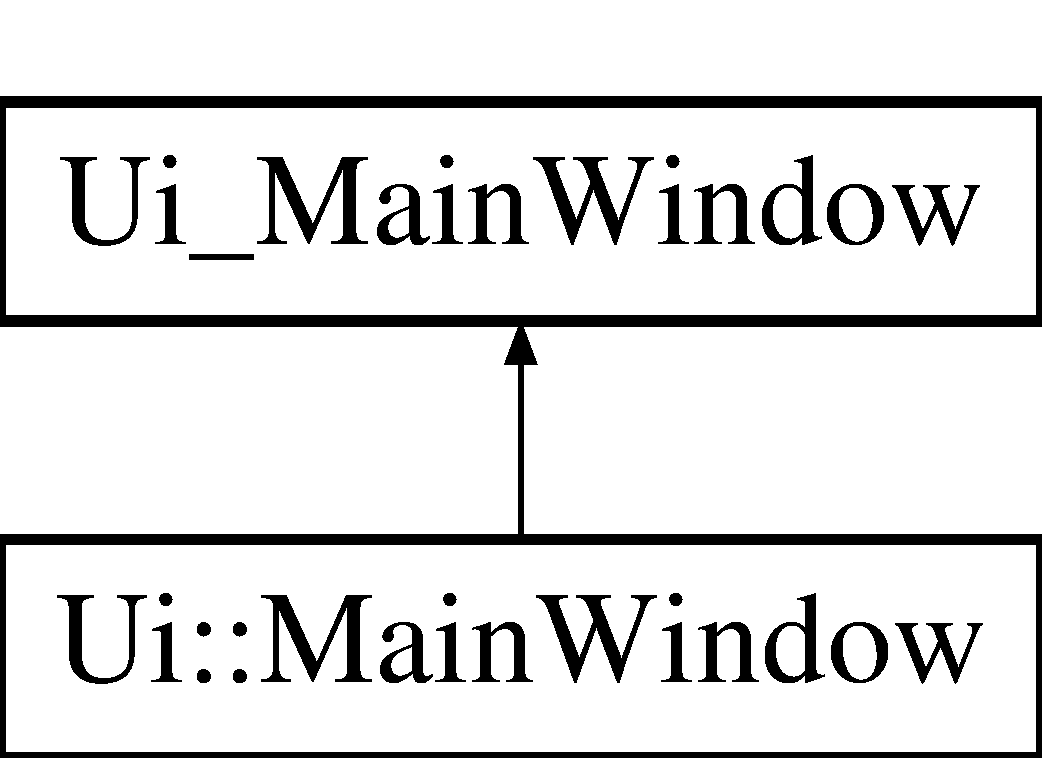
\includegraphics[height=2.000000cm]{class_ui_1_1_main_window}
\end{center}
\end{figure}
\subsection*{Additional Inherited Members}


The documentation for this class was generated from the following file\-:\begin{DoxyCompactItemize}
\item 
/home/aaiiighht/\-Bureau/projet\-T\-L/automate-\/project/ui\-\_\-mainwindow.\-h\end{DoxyCompactItemize}

\hypertarget{class_main_window}{\section{Main\-Window Class Reference}
\label{class_main_window}\index{Main\-Window@{Main\-Window}}
}
Inheritance diagram for Main\-Window\-:\begin{figure}[H]
\begin{center}
\leavevmode
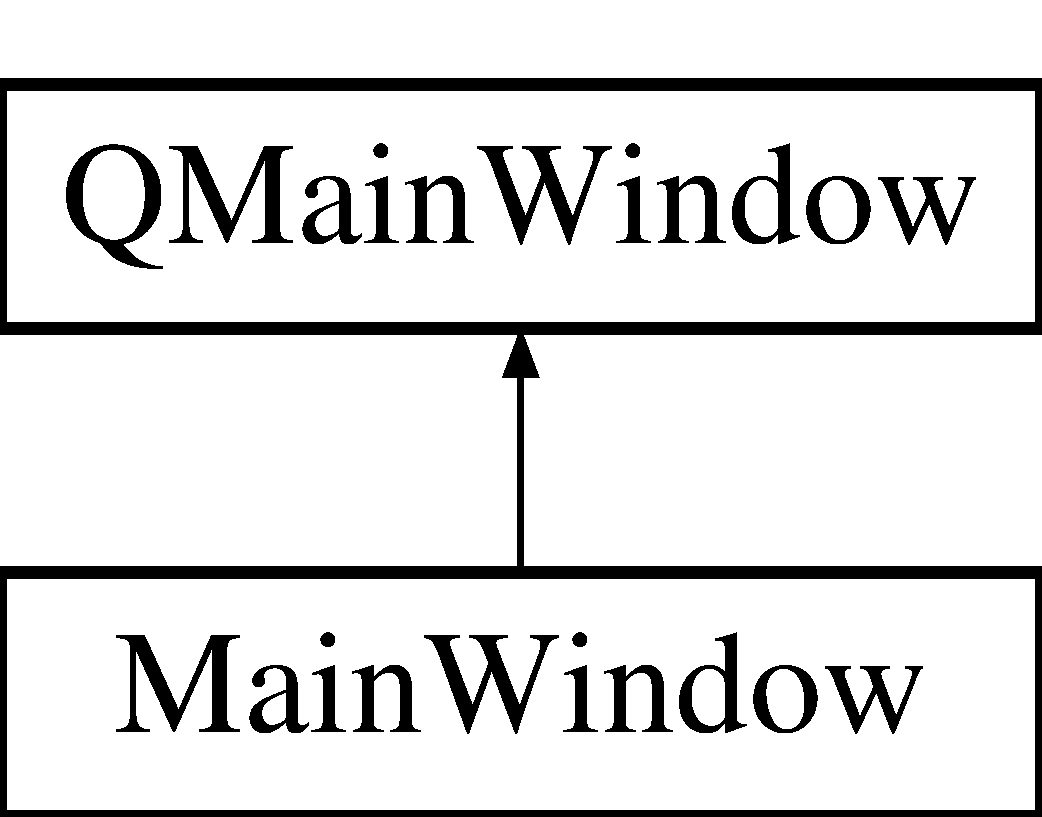
\includegraphics[height=2.000000cm]{class_main_window}
\end{center}
\end{figure}
\subsection*{Public Slots}
\begin{DoxyCompactItemize}
\item 
void \hyperlink{class_main_window_a288b768c3c21a9171bdc56fe845ece8b}{open\-File} ()
\begin{DoxyCompactList}\small\item\em Permet d'ouvrir un automate, stocké dans un fichier .dot. \end{DoxyCompactList}\item 
void \hyperlink{class_main_window_afc3b7768c20897733c1097fb5d956a6d}{creer\-Auto} ()
\begin{DoxyCompactList}\small\item\em Permet d'accéder à la fenêtre de création d'automate. \end{DoxyCompactList}\item 
void \hyperlink{class_main_window_a2b49ea4a32d41b1a5a60c8d3b844a122}{get\-Produit} ()
\begin{DoxyCompactList}\small\item\em Permet de faire le produit de 2 automates. \end{DoxyCompactList}\item 
void \hyperlink{class_main_window_ada476693941f6f33c5ec3c6089ec4058}{get\-Determin} ()
\begin{DoxyCompactList}\small\item\em Permet de déterminiser un automate. \end{DoxyCompactList}\item 
void \hyperlink{class_main_window_a5163f212156eecd4624ced33f1574361}{get\-Suivant} ()
\begin{DoxyCompactList}\small\item\em Permet de passer à l'étape suivant pour une des opérations. \end{DoxyCompactList}\item 
void \hyperlink{class_main_window_ad3f7fb432b87dd1c613d678cbc2b36fe}{get\-Precedent} ()
\begin{DoxyCompactList}\small\item\em Permet de passer à l'étape précédente pour une des opérations. \end{DoxyCompactList}\item 
void \hyperlink{class_main_window_a8743d62b3db7581d930b2b8faa852ca7}{get\-Standard} ()
\begin{DoxyCompactList}\small\item\em Permet de standardiser un automate. \end{DoxyCompactList}\item 
void \hyperlink{class_main_window_ae81811139b9d004b68f5654ad40a7b52}{get\-Minimisation} ()
\begin{DoxyCompactList}\small\item\em Permet de minimiser un automate. \end{DoxyCompactList}\item 
void \hyperlink{class_main_window_ae0830e3c5a46ae29d7fd9cc870fe6c08}{reset\-Ui} ()
\begin{DoxyCompactList}\small\item\em Permet de nettoyer la fenetre. \end{DoxyCompactList}\item 
\hypertarget{class_main_window_adef6f7c5939e0e2b60414a55d716ddc8}{void {\bfseries test} ()}\label{class_main_window_adef6f7c5939e0e2b60414a55d716ddc8}

\item 
void \hyperlink{class_main_window_a78f945084286506a64269d4ee75db224}{info} ()
\begin{DoxyCompactList}\small\item\em Permet d'afficher des informations sur les boutons et le fonctionnement du logiciel. \end{DoxyCompactList}\end{DoxyCompactItemize}
\subsection*{Public Member Functions}
\begin{DoxyCompactItemize}
\item 
\hyperlink{class_main_window_a8b244be8b7b7db1b08de2a2acb9409db}{Main\-Window} (Q\-Widget $\ast$parent=0)
\begin{DoxyCompactList}\small\item\em Constructeur. \end{DoxyCompactList}\item 
\hyperlink{class_main_window_ae98d00a93bc118200eeef9f9bba1dba7}{$\sim$\-Main\-Window} ()
\begin{DoxyCompactList}\small\item\em Destructeur. \end{DoxyCompactList}\item 
\hypertarget{class_main_window_a22ccaf0f029e895977c18774bf9ef115}{void {\bfseries start\-Layouting} ()}\label{class_main_window_a22ccaf0f029e895977c18774bf9ef115}

\item 
\hypertarget{class_main_window_ac9f5af352ce35293a2246f28af46b88c}{void {\bfseries affiche\-Automate} (\hyperlink{class_automate}{Automate})}\label{class_main_window_ac9f5af352ce35293a2246f28af46b88c}

\item 
\hypertarget{class_main_window_a7c730609e4e9f30d1b2dc88f8762a05c}{bool {\bfseries lire\-Dot} ()}\label{class_main_window_a7c730609e4e9f30d1b2dc88f8762a05c}

\item 
\hypertarget{class_main_window_ac9ec17b8cd9fe73a0cddfdc4423c9fb3}{bool {\bfseries lire\-Dot\-B} ()}\label{class_main_window_ac9ec17b8cd9fe73a0cddfdc4423c9fb3}

\end{DoxyCompactItemize}
\subsection*{Public Attributes}
\begin{DoxyCompactItemize}
\item 
\hypertarget{class_main_window_afe417a179b1efb0d372b4f8662cdd8e2}{Q\-Process $\ast$ {\bfseries Process\-T}}\label{class_main_window_afe417a179b1efb0d372b4f8662cdd8e2}

\item 
\hypertarget{class_main_window_a8edeaf68e7fac9c43d4b0cec2b859e90}{Q\-String {\bfseries program}}\label{class_main_window_a8edeaf68e7fac9c43d4b0cec2b859e90}

\end{DoxyCompactItemize}
\subsection*{Protected Member Functions}
\begin{DoxyCompactItemize}
\item 
\hypertarget{class_main_window_af4ca5d0d3d18ddcb7d54b6596bbf4797}{void {\bfseries change\-Event} (Q\-Event $\ast$e)}\label{class_main_window_af4ca5d0d3d18ddcb7d54b6596bbf4797}

\end{DoxyCompactItemize}


\subsection{Constructor \& Destructor Documentation}
\hypertarget{class_main_window_a8b244be8b7b7db1b08de2a2acb9409db}{\index{Main\-Window@{Main\-Window}!Main\-Window@{Main\-Window}}
\index{Main\-Window@{Main\-Window}!MainWindow@{Main\-Window}}
\subsubsection[{Main\-Window}]{\setlength{\rightskip}{0pt plus 5cm}Main\-Window\-::\-Main\-Window (
\begin{DoxyParamCaption}
\item[{Q\-Widget $\ast$}]{parent = {\ttfamily 0}}
\end{DoxyParamCaption}
)}}\label{class_main_window_a8b244be8b7b7db1b08de2a2acb9409db}


Constructeur. 

Construit la fenetre. \hypertarget{class_main_window_ae98d00a93bc118200eeef9f9bba1dba7}{\index{Main\-Window@{Main\-Window}!$\sim$\-Main\-Window@{$\sim$\-Main\-Window}}
\index{$\sim$\-Main\-Window@{$\sim$\-Main\-Window}!MainWindow@{Main\-Window}}
\subsubsection[{$\sim$\-Main\-Window}]{\setlength{\rightskip}{0pt plus 5cm}Main\-Window\-::$\sim$\-Main\-Window (
\begin{DoxyParamCaption}
{}
\end{DoxyParamCaption}
)}}\label{class_main_window_ae98d00a93bc118200eeef9f9bba1dba7}


Destructeur. 

Destructeur de la classe \hyperlink{class_main_window}{Main\-Window} 

\subsection{Member Function Documentation}
\hypertarget{class_main_window_afc3b7768c20897733c1097fb5d956a6d}{\index{Main\-Window@{Main\-Window}!creer\-Auto@{creer\-Auto}}
\index{creer\-Auto@{creer\-Auto}!MainWindow@{Main\-Window}}
\subsubsection[{creer\-Auto}]{\setlength{\rightskip}{0pt plus 5cm}void Main\-Window\-::creer\-Auto (
\begin{DoxyParamCaption}
{}
\end{DoxyParamCaption}
)\hspace{0.3cm}{\ttfamily [slot]}}}\label{class_main_window_afc3b7768c20897733c1097fb5d956a6d}


Permet d'accéder à la fenêtre de création d'automate. 

Listener du bouton ouvrir un automate, propose une fenetre pour créer un automate. \hypertarget{class_main_window_ada476693941f6f33c5ec3c6089ec4058}{\index{Main\-Window@{Main\-Window}!get\-Determin@{get\-Determin}}
\index{get\-Determin@{get\-Determin}!MainWindow@{Main\-Window}}
\subsubsection[{get\-Determin}]{\setlength{\rightskip}{0pt plus 5cm}void Main\-Window\-::get\-Determin (
\begin{DoxyParamCaption}
{}
\end{DoxyParamCaption}
)\hspace{0.3cm}{\ttfamily [slot]}}}\label{class_main_window_ada476693941f6f33c5ec3c6089ec4058}


Permet de déterminiser un automate. 

Listener du bouton déterminiser. L'automate ouvert sera affiché dans ma\-Vue1. L'automate résultat du produit affiché dans ma\-Vue. \hypertarget{class_main_window_ae81811139b9d004b68f5654ad40a7b52}{\index{Main\-Window@{Main\-Window}!get\-Minimisation@{get\-Minimisation}}
\index{get\-Minimisation@{get\-Minimisation}!MainWindow@{Main\-Window}}
\subsubsection[{get\-Minimisation}]{\setlength{\rightskip}{0pt plus 5cm}void Main\-Window\-::get\-Minimisation (
\begin{DoxyParamCaption}
{}
\end{DoxyParamCaption}
)\hspace{0.3cm}{\ttfamily [slot]}}}\label{class_main_window_ae81811139b9d004b68f5654ad40a7b52}


Permet de minimiser un automate. 

Listener du bouton minimiser. L'automate ouvert sera affiché dans ma\-Vue1. L'automate résultat du produit affiché dans ma\-Vue. \hypertarget{class_main_window_ad3f7fb432b87dd1c613d678cbc2b36fe}{\index{Main\-Window@{Main\-Window}!get\-Precedent@{get\-Precedent}}
\index{get\-Precedent@{get\-Precedent}!MainWindow@{Main\-Window}}
\subsubsection[{get\-Precedent}]{\setlength{\rightskip}{0pt plus 5cm}void Main\-Window\-::get\-Precedent (
\begin{DoxyParamCaption}
{}
\end{DoxyParamCaption}
)\hspace{0.3cm}{\ttfamily [slot]}}}\label{class_main_window_ad3f7fb432b87dd1c613d678cbc2b36fe}


Permet de passer à l'étape précédente pour une des opérations. 

Listener du bouton précédent. L'étape précédente, s'il y en a une, d'une des opérations (standardisation, produit etc) sera affichée au lieu de l'actuel. \hypertarget{class_main_window_a2b49ea4a32d41b1a5a60c8d3b844a122}{\index{Main\-Window@{Main\-Window}!get\-Produit@{get\-Produit}}
\index{get\-Produit@{get\-Produit}!MainWindow@{Main\-Window}}
\subsubsection[{get\-Produit}]{\setlength{\rightskip}{0pt plus 5cm}void Main\-Window\-::get\-Produit (
\begin{DoxyParamCaption}
{}
\end{DoxyParamCaption}
)\hspace{0.3cm}{\ttfamily [slot]}}}\label{class_main_window_a2b49ea4a32d41b1a5a60c8d3b844a122}


Permet de faire le produit de 2 automates. 

Listener du bouton faire le produit de 2 automates, propose d'abord d'ouvrir une fenetre pour afficher le second automate. L'automate déjà ouvert sera affiché dans ma\-Vue1. L'automate ouvert sera affiché dans ma\-Vue2. L'automate résultat du produit sera affiché dans ma\-Vue. \hypertarget{class_main_window_a8743d62b3db7581d930b2b8faa852ca7}{\index{Main\-Window@{Main\-Window}!get\-Standard@{get\-Standard}}
\index{get\-Standard@{get\-Standard}!MainWindow@{Main\-Window}}
\subsubsection[{get\-Standard}]{\setlength{\rightskip}{0pt plus 5cm}void Main\-Window\-::get\-Standard (
\begin{DoxyParamCaption}
{}
\end{DoxyParamCaption}
)\hspace{0.3cm}{\ttfamily [slot]}}}\label{class_main_window_a8743d62b3db7581d930b2b8faa852ca7}


Permet de standardiser un automate. 

Listener du bouton standardiser. L'automate ouvert sera affiché dans ma\-Vue1. L'automate résultat du produit affiché dans ma\-Vue. \hypertarget{class_main_window_a5163f212156eecd4624ced33f1574361}{\index{Main\-Window@{Main\-Window}!get\-Suivant@{get\-Suivant}}
\index{get\-Suivant@{get\-Suivant}!MainWindow@{Main\-Window}}
\subsubsection[{get\-Suivant}]{\setlength{\rightskip}{0pt plus 5cm}void Main\-Window\-::get\-Suivant (
\begin{DoxyParamCaption}
{}
\end{DoxyParamCaption}
)\hspace{0.3cm}{\ttfamily [slot]}}}\label{class_main_window_a5163f212156eecd4624ced33f1574361}


Permet de passer à l'étape suivant pour une des opérations. 

Listener du bouton suivant. L'étape suivante, s'il y en a une, d'une des opérations (standardisation, produit etc) sera affichée au lieu de l'actuel. \hypertarget{class_main_window_a78f945084286506a64269d4ee75db224}{\index{Main\-Window@{Main\-Window}!info@{info}}
\index{info@{info}!MainWindow@{Main\-Window}}
\subsubsection[{info}]{\setlength{\rightskip}{0pt plus 5cm}void Main\-Window\-::info (
\begin{DoxyParamCaption}
{}
\end{DoxyParamCaption}
)\hspace{0.3cm}{\ttfamily [slot]}}}\label{class_main_window_a78f945084286506a64269d4ee75db224}


Permet d'afficher des informations sur les boutons et le fonctionnement du logiciel. 

Listener du bouton Info. Affiche dans la fenetre de droite des informations sur les boutons \hypertarget{class_main_window_a288b768c3c21a9171bdc56fe845ece8b}{\index{Main\-Window@{Main\-Window}!open\-File@{open\-File}}
\index{open\-File@{open\-File}!MainWindow@{Main\-Window}}
\subsubsection[{open\-File}]{\setlength{\rightskip}{0pt plus 5cm}void Main\-Window\-::open\-File (
\begin{DoxyParamCaption}
{}
\end{DoxyParamCaption}
)\hspace{0.3cm}{\ttfamily [slot]}}}\label{class_main_window_a288b768c3c21a9171bdc56fe845ece8b}


Permet d'ouvrir un automate, stocké dans un fichier .dot. 

Listener du bouton ouvrir un automate, propose une fenetre pour sélectionner un fichier .dot correspondant à un automate. Cet automate sera ensuite afficher dans ma\-Vue \hypertarget{class_main_window_ae0830e3c5a46ae29d7fd9cc870fe6c08}{\index{Main\-Window@{Main\-Window}!reset\-Ui@{reset\-Ui}}
\index{reset\-Ui@{reset\-Ui}!MainWindow@{Main\-Window}}
\subsubsection[{reset\-Ui}]{\setlength{\rightskip}{0pt plus 5cm}void Main\-Window\-::reset\-Ui (
\begin{DoxyParamCaption}
{}
\end{DoxyParamCaption}
)\hspace{0.3cm}{\ttfamily [slot]}}}\label{class_main_window_ae0830e3c5a46ae29d7fd9cc870fe6c08}


Permet de nettoyer la fenetre. 

Listener du bouton nettoyer l'interface. Vide la fenetre et la ramène à un état comme au démarrage de l'application 

The documentation for this class was generated from the following files\-:\begin{DoxyCompactItemize}
\item 
/home/aaiiighht/\-Bureau/projet\-T\-L/automate-\/project/\hyperlink{mainwindow_8h}{mainwindow.\-h}\item 
/home/aaiiighht/\-Bureau/projet\-T\-L/automate-\/project/mainwindow.\-cpp\end{DoxyCompactItemize}

\hypertarget{structqt__meta__stringdata__choix_pointe__t}{\section{qt\-\_\-meta\-\_\-stringdata\-\_\-choix\-Pointe\-\_\-t Struct Reference}
\label{structqt__meta__stringdata__choix_pointe__t}\index{qt\-\_\-meta\-\_\-stringdata\-\_\-choix\-Pointe\-\_\-t@{qt\-\_\-meta\-\_\-stringdata\-\_\-choix\-Pointe\-\_\-t}}
}
\subsection*{Public Attributes}
\begin{DoxyCompactItemize}
\item 
\hypertarget{structqt__meta__stringdata__choix_pointe__t_ad3b353765e9d7e892b76492d283369d8}{Q\-Byte\-Array\-Data {\bfseries data} \mbox{[}6\mbox{]}}\label{structqt__meta__stringdata__choix_pointe__t_ad3b353765e9d7e892b76492d283369d8}

\item 
\hypertarget{structqt__meta__stringdata__choix_pointe__t_afc6132c465afb6133de2cea8933ef830}{char {\bfseries stringdata} \mbox{[}38\mbox{]}}\label{structqt__meta__stringdata__choix_pointe__t_afc6132c465afb6133de2cea8933ef830}

\end{DoxyCompactItemize}


The documentation for this struct was generated from the following file\-:\begin{DoxyCompactItemize}
\item 
/home/aaiiighht/\-Bureau/projet\-T\-L/automate-\/project/moc\-\_\-choixpointe.\-cpp\end{DoxyCompactItemize}

\hypertarget{structqt__meta__stringdata___create_automate__t}{\section{qt\-\_\-meta\-\_\-stringdata\-\_\-\-Create\-Automate\-\_\-t Struct Reference}
\label{structqt__meta__stringdata___create_automate__t}\index{qt\-\_\-meta\-\_\-stringdata\-\_\-\-Create\-Automate\-\_\-t@{qt\-\_\-meta\-\_\-stringdata\-\_\-\-Create\-Automate\-\_\-t}}
}
\subsection*{Public Attributes}
\begin{DoxyCompactItemize}
\item 
\hypertarget{structqt__meta__stringdata___create_automate__t_a210bd9798698d39b50889826c7b0cdc4}{Q\-Byte\-Array\-Data {\bfseries data} \mbox{[}11\mbox{]}}\label{structqt__meta__stringdata___create_automate__t_a210bd9798698d39b50889826c7b0cdc4}

\item 
\hypertarget{structqt__meta__stringdata___create_automate__t_ad815d5cc87bba2f46cb82e58f587d01c}{char {\bfseries stringdata} \mbox{[}114\mbox{]}}\label{structqt__meta__stringdata___create_automate__t_ad815d5cc87bba2f46cb82e58f587d01c}

\end{DoxyCompactItemize}


The documentation for this struct was generated from the following file\-:\begin{DoxyCompactItemize}
\item 
/home/aaiiighht/\-Bureau/smartgit/bin/projet\-T\-L/automate-\/project/moc\-\_\-createautomate.\-cpp\end{DoxyCompactItemize}

\hypertarget{structqt__meta__stringdata__etat_left__t}{\section{qt\-\_\-meta\-\_\-stringdata\-\_\-etat\-Left\-\_\-t Struct Reference}
\label{structqt__meta__stringdata__etat_left__t}\index{qt\-\_\-meta\-\_\-stringdata\-\_\-etat\-Left\-\_\-t@{qt\-\_\-meta\-\_\-stringdata\-\_\-etat\-Left\-\_\-t}}
}
\subsection*{Public Attributes}
\begin{DoxyCompactItemize}
\item 
\hypertarget{structqt__meta__stringdata__etat_left__t_ad16d3d553795be640d70bc3f777ad44c}{Q\-Byte\-Array\-Data {\bfseries data} \mbox{[}7\mbox{]}}\label{structqt__meta__stringdata__etat_left__t_ad16d3d553795be640d70bc3f777ad44c}

\item 
\hypertarget{structqt__meta__stringdata__etat_left__t_a091074801566ffe89515b5a1b998903e}{char {\bfseries stringdata} \mbox{[}53\mbox{]}}\label{structqt__meta__stringdata__etat_left__t_a091074801566ffe89515b5a1b998903e}

\end{DoxyCompactItemize}


The documentation for this struct was generated from the following file\-:\begin{DoxyCompactItemize}
\item 
/home/aaiiighht/\-Bureau/smartgit/bin/projet\-T\-L/automate-\/project/moc\-\_\-etatleft.\-cpp\end{DoxyCompactItemize}

\hypertarget{structqt__meta__stringdata__etat_right__t}{\section{qt\-\_\-meta\-\_\-stringdata\-\_\-etat\-Right\-\_\-t Struct Reference}
\label{structqt__meta__stringdata__etat_right__t}\index{qt\-\_\-meta\-\_\-stringdata\-\_\-etat\-Right\-\_\-t@{qt\-\_\-meta\-\_\-stringdata\-\_\-etat\-Right\-\_\-t}}
}
\subsection*{Public Attributes}
\begin{DoxyCompactItemize}
\item 
\hypertarget{structqt__meta__stringdata__etat_right__t_a3df3a504f319e535d278c0520a3365a5}{Q\-Byte\-Array\-Data {\bfseries data} \mbox{[}7\mbox{]}}\label{structqt__meta__stringdata__etat_right__t_a3df3a504f319e535d278c0520a3365a5}

\item 
\hypertarget{structqt__meta__stringdata__etat_right__t_abb73320c6aab80e726ee5fcf933bc1fb}{char {\bfseries stringdata} \mbox{[}79\mbox{]}}\label{structqt__meta__stringdata__etat_right__t_abb73320c6aab80e726ee5fcf933bc1fb}

\end{DoxyCompactItemize}


The documentation for this struct was generated from the following file\-:\begin{DoxyCompactItemize}
\item 
/home/aaiiighht/\-Bureau/projet\-T\-L/automate-\/project/moc\-\_\-etatright.\-cpp\end{DoxyCompactItemize}

\hypertarget{structqt__meta__stringdata___main_window__t}{\section{qt\-\_\-meta\-\_\-stringdata\-\_\-\-Main\-Window\-\_\-t Struct Reference}
\label{structqt__meta__stringdata___main_window__t}\index{qt\-\_\-meta\-\_\-stringdata\-\_\-\-Main\-Window\-\_\-t@{qt\-\_\-meta\-\_\-stringdata\-\_\-\-Main\-Window\-\_\-t}}
}
\subsection*{Public Attributes}
\begin{DoxyCompactItemize}
\item 
\hypertarget{structqt__meta__stringdata___main_window__t_a3425efb15419da867ddd69f8a4ed9e67}{Q\-Byte\-Array\-Data {\bfseries data} \mbox{[}13\mbox{]}}\label{structqt__meta__stringdata___main_window__t_a3425efb15419da867ddd69f8a4ed9e67}

\item 
\hypertarget{structqt__meta__stringdata___main_window__t_a83a4e6119d3600df5ed2ecd99c255853}{char {\bfseries stringdata} \mbox{[}125\mbox{]}}\label{structqt__meta__stringdata___main_window__t_a83a4e6119d3600df5ed2ecd99c255853}

\end{DoxyCompactItemize}


The documentation for this struct was generated from the following file\-:\begin{DoxyCompactItemize}
\item 
/home/aaiiighht/\-Bureau/projet\-T\-L/automate-\/project/moc\-\_\-mainwindow.\-cpp\end{DoxyCompactItemize}

\hypertarget{structqt__meta__stringdata___transition__t}{\section{qt\-\_\-meta\-\_\-stringdata\-\_\-\-Transition\-\_\-t Struct Reference}
\label{structqt__meta__stringdata___transition__t}\index{qt\-\_\-meta\-\_\-stringdata\-\_\-\-Transition\-\_\-t@{qt\-\_\-meta\-\_\-stringdata\-\_\-\-Transition\-\_\-t}}
}
\subsection*{Public Attributes}
\begin{DoxyCompactItemize}
\item 
\hypertarget{structqt__meta__stringdata___transition__t_a420f3dc424f227b1518aaa09fbf40b72}{Q\-Byte\-Array\-Data {\bfseries data} \mbox{[}4\mbox{]}}\label{structqt__meta__stringdata___transition__t_a420f3dc424f227b1518aaa09fbf40b72}

\item 
\hypertarget{structqt__meta__stringdata___transition__t_a99978081bcceecad4629a80f196be3a6}{char {\bfseries stringdata} \mbox{[}27\mbox{]}}\label{structqt__meta__stringdata___transition__t_a99978081bcceecad4629a80f196be3a6}

\end{DoxyCompactItemize}


The documentation for this struct was generated from the following file\-:\begin{DoxyCompactItemize}
\item 
/home/aaiiighht/\-Bureau/projet\-T\-L/automate-\/project/moc\-\_\-transition.\-cpp\end{DoxyCompactItemize}

\hypertarget{class_ui_1_1_transition}{\section{Ui\-:\-:Transition Class Reference}
\label{class_ui_1_1_transition}\index{Ui\-::\-Transition@{Ui\-::\-Transition}}
}


Inheritance diagram for Ui\-:\-:Transition\-:
\nopagebreak
\begin{figure}[H]
\begin{center}
\leavevmode
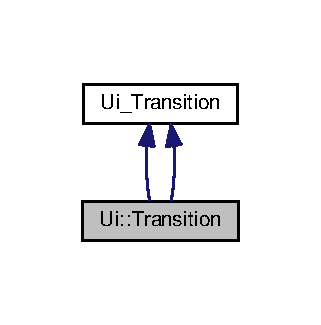
\includegraphics[width=154pt]{class_ui_1_1_transition__inherit__graph}
\end{center}
\end{figure}


Collaboration diagram for Ui\-:\-:Transition\-:
\nopagebreak
\begin{figure}[H]
\begin{center}
\leavevmode
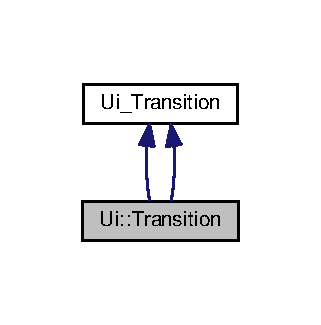
\includegraphics[width=154pt]{class_ui_1_1_transition__coll__graph}
\end{center}
\end{figure}
\subsection*{Additional Inherited Members}


The documentation for this class was generated from the following file\-:\begin{DoxyCompactItemize}
\item 
/home/aaiiighht/\-Bureau/smartgit/bin/projet\-T\-L/automate-\/project/release/ui\-\_\-transition.\-h\end{DoxyCompactItemize}

\hypertarget{class_transition}{\section{Transition Class Reference}
\label{class_transition}\index{Transition@{Transition}}
}


Inheritance diagram for Transition\-:
\nopagebreak
\begin{figure}[H]
\begin{center}
\leavevmode
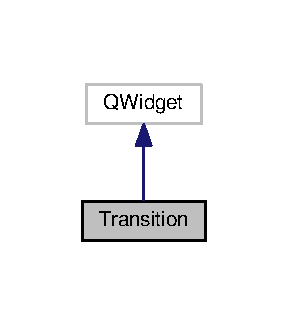
\includegraphics[width=138pt]{class_transition__inherit__graph}
\end{center}
\end{figure}


Collaboration diagram for Transition\-:
\nopagebreak
\begin{figure}[H]
\begin{center}
\leavevmode
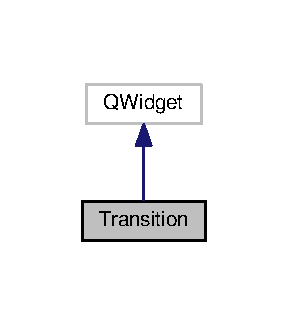
\includegraphics[width=138pt]{class_transition__coll__graph}
\end{center}
\end{figure}
\subsection*{Public Slots}
\begin{DoxyCompactItemize}
\item 
\hypertarget{class_transition_a74d10ea64197661946db6d02b35b4cf1}{void {\bfseries get\-Off} ()}\label{class_transition_a74d10ea64197661946db6d02b35b4cf1}

\end{DoxyCompactItemize}
\subsection*{Signals}
\begin{DoxyCompactItemize}
\item 
\hypertarget{class_transition_abbd3e6ff526c19cd4ebc629d1be10200}{void {\bfseries eraser} (int, int)}\label{class_transition_abbd3e6ff526c19cd4ebc629d1be10200}

\end{DoxyCompactItemize}
\subsection*{Public Member Functions}
\begin{DoxyCompactItemize}
\item 
\hypertarget{class_transition_a42b17d24af24110d405ce53c1956cc2e}{{\bfseries Transition} (int, int, Q\-Widget $\ast$parent=0)}\label{class_transition_a42b17d24af24110d405ce53c1956cc2e}

\end{DoxyCompactItemize}
\subsection*{Public Attributes}
\begin{DoxyCompactItemize}
\item 
\hypertarget{class_transition_a1b3f80305749c8f032a7f711527b0fc3}{int {\bfseries cible}}\label{class_transition_a1b3f80305749c8f032a7f711527b0fc3}

\item 
\hypertarget{class_transition_a209c68fd432cd8e763342c1f2c784a87}{int {\bfseries vocab}}\label{class_transition_a209c68fd432cd8e763342c1f2c784a87}

\end{DoxyCompactItemize}
\subsection*{Protected Member Functions}
\begin{DoxyCompactItemize}
\item 
\hypertarget{class_transition_a9df49098a20b28bd720e96d69255a026}{void {\bfseries change\-Event} (Q\-Event $\ast$e)}\label{class_transition_a9df49098a20b28bd720e96d69255a026}

\end{DoxyCompactItemize}


The documentation for this class was generated from the following files\-:\begin{DoxyCompactItemize}
\item 
/home/aaiiighht/\-Bureau/smartgit/bin/projet\-T\-L/automate-\/project/transition.\-h\item 
/home/aaiiighht/\-Bureau/smartgit/bin/projet\-T\-L/automate-\/project/debug/moc\-\_\-transition.\-cpp\item 
/home/aaiiighht/\-Bureau/smartgit/bin/projet\-T\-L/automate-\/project/transition.\-cpp\end{DoxyCompactItemize}

\hypertarget{class_ui__choix_pointe}{\section{Ui\-\_\-choix\-Pointe Class Reference}
\label{class_ui__choix_pointe}\index{Ui\-\_\-choix\-Pointe@{Ui\-\_\-choix\-Pointe}}
}


Inheritance diagram for Ui\-\_\-choix\-Pointe\-:
\nopagebreak
\begin{figure}[H]
\begin{center}
\leavevmode
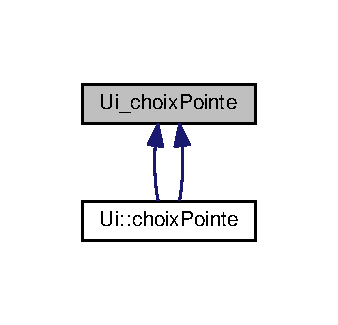
\includegraphics[width=162pt]{class_ui__choix_pointe__inherit__graph}
\end{center}
\end{figure}
\subsection*{Public Member Functions}
\begin{DoxyCompactItemize}
\item 
\hypertarget{class_ui__choix_pointe_afb01f288ce6a40c26c0346d1e0024f4e}{void {\bfseries setup\-Ui} (Q\-Widget $\ast$\hyperlink{classchoix_pointe}{choix\-Pointe})}\label{class_ui__choix_pointe_afb01f288ce6a40c26c0346d1e0024f4e}

\item 
\hypertarget{class_ui__choix_pointe_aea42cc3aeeb1ea76b18aeac75a7ec2cc}{void {\bfseries retranslate\-Ui} (Q\-Widget $\ast$\hyperlink{classchoix_pointe}{choix\-Pointe})}\label{class_ui__choix_pointe_aea42cc3aeeb1ea76b18aeac75a7ec2cc}

\item 
\hypertarget{class_ui__choix_pointe_afb01f288ce6a40c26c0346d1e0024f4e}{void {\bfseries setup\-Ui} (Q\-Widget $\ast$\hyperlink{classchoix_pointe}{choix\-Pointe})}\label{class_ui__choix_pointe_afb01f288ce6a40c26c0346d1e0024f4e}

\item 
\hypertarget{class_ui__choix_pointe_aea42cc3aeeb1ea76b18aeac75a7ec2cc}{void {\bfseries retranslate\-Ui} (Q\-Widget $\ast$\hyperlink{classchoix_pointe}{choix\-Pointe})}\label{class_ui__choix_pointe_aea42cc3aeeb1ea76b18aeac75a7ec2cc}

\end{DoxyCompactItemize}
\subsection*{Public Attributes}
\begin{DoxyCompactItemize}
\item 
\hypertarget{class_ui__choix_pointe_a7afdfea5e8c527bd48b8dcf812e9313b}{Q\-V\-Box\-Layout $\ast$ {\bfseries vertical\-Layout\-\_\-2}}\label{class_ui__choix_pointe_a7afdfea5e8c527bd48b8dcf812e9313b}

\item 
\hypertarget{class_ui__choix_pointe_a2a1342e3137752c3a24a8a8c81b87331}{Q\-Frame $\ast$ {\bfseries Widget}}\label{class_ui__choix_pointe_a2a1342e3137752c3a24a8a8c81b87331}

\item 
\hypertarget{class_ui__choix_pointe_aeabb6c9ebcf9467663fdc530c0bb4237}{Q\-H\-Box\-Layout $\ast$ {\bfseries horizontal\-Layout}}\label{class_ui__choix_pointe_aeabb6c9ebcf9467663fdc530c0bb4237}

\item 
\hypertarget{class_ui__choix_pointe_a1930f2367ebc807106aa83407ac8362f}{Q\-Label $\ast$ {\bfseries label\-\_\-3}}\label{class_ui__choix_pointe_a1930f2367ebc807106aa83407ac8362f}

\item 
\hypertarget{class_ui__choix_pointe_afe24a2593c7263dd1f914bcd64b54c41}{Q\-Combo\-Box $\ast$ {\bfseries les\-Choix}}\label{class_ui__choix_pointe_afe24a2593c7263dd1f914bcd64b54c41}

\item 
\hypertarget{class_ui__choix_pointe_aa0913ec085e3bcd801ce0e1d0a3cc9c9}{Q\-Label $\ast$ {\bfseries label\-\_\-4}}\label{class_ui__choix_pointe_aa0913ec085e3bcd801ce0e1d0a3cc9c9}

\item 
\hypertarget{class_ui__choix_pointe_a8b9faf280027191a0d777b165edcbf1c}{Q\-Line\-Edit $\ast$ {\bfseries line\-Edit}}\label{class_ui__choix_pointe_a8b9faf280027191a0d777b165edcbf1c}

\item 
\hypertarget{class_ui__choix_pointe_a07dc96c47c44081ff741dfdb827607e5}{Q\-Push\-Button $\ast$ {\bfseries push\-Button}}\label{class_ui__choix_pointe_a07dc96c47c44081ff741dfdb827607e5}

\end{DoxyCompactItemize}


The documentation for this class was generated from the following file\-:\begin{DoxyCompactItemize}
\item 
/home/aaiiighht/\-Bureau/smartgit/bin/projet\-T\-L/automate-\/project/release/ui\-\_\-choixpointe.\-h\end{DoxyCompactItemize}

\hypertarget{class_ui___create_automate}{\section{Ui\-\_\-\-Create\-Automate Class Reference}
\label{class_ui___create_automate}\index{Ui\-\_\-\-Create\-Automate@{Ui\-\_\-\-Create\-Automate}}
}


Inheritance diagram for Ui\-\_\-\-Create\-Automate\-:
\nopagebreak
\begin{figure}[H]
\begin{center}
\leavevmode
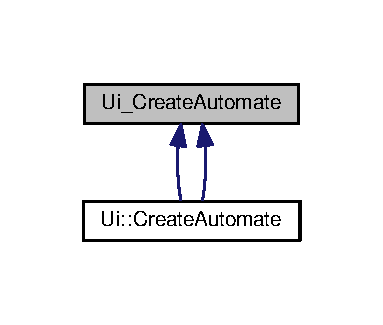
\includegraphics[width=184pt]{class_ui___create_automate__inherit__graph}
\end{center}
\end{figure}
\subsection*{Public Member Functions}
\begin{DoxyCompactItemize}
\item 
\hypertarget{class_ui___create_automate_adc1c604839808d7f0699c4c2075d119c}{void {\bfseries setup\-Ui} (Q\-Main\-Window $\ast$\hyperlink{class_create_automate}{Create\-Automate})}\label{class_ui___create_automate_adc1c604839808d7f0699c4c2075d119c}

\item 
\hypertarget{class_ui___create_automate_ac995057d86d1b7fd1f805ea116112e82}{void {\bfseries retranslate\-Ui} (Q\-Main\-Window $\ast$\hyperlink{class_create_automate}{Create\-Automate})}\label{class_ui___create_automate_ac995057d86d1b7fd1f805ea116112e82}

\item 
\hypertarget{class_ui___create_automate_adc1c604839808d7f0699c4c2075d119c}{void {\bfseries setup\-Ui} (Q\-Main\-Window $\ast$\hyperlink{class_create_automate}{Create\-Automate})}\label{class_ui___create_automate_adc1c604839808d7f0699c4c2075d119c}

\item 
\hypertarget{class_ui___create_automate_ac995057d86d1b7fd1f805ea116112e82}{void {\bfseries retranslate\-Ui} (Q\-Main\-Window $\ast$\hyperlink{class_create_automate}{Create\-Automate})}\label{class_ui___create_automate_ac995057d86d1b7fd1f805ea116112e82}

\end{DoxyCompactItemize}
\subsection*{Public Attributes}
\begin{DoxyCompactItemize}
\item 
\hypertarget{class_ui___create_automate_ab640344ed172ed3b3f99fc20dfca4ccd}{Q\-Action $\ast$ {\bfseries action\-Fermer}}\label{class_ui___create_automate_ab640344ed172ed3b3f99fc20dfca4ccd}

\item 
\hypertarget{class_ui___create_automate_a589a8428623e28a3099d25a54e6f5beb}{Q\-Action $\ast$ {\bfseries action\-Voir}}\label{class_ui___create_automate_a589a8428623e28a3099d25a54e6f5beb}

\item 
\hypertarget{class_ui___create_automate_a8f114b81317ce3fd1882aba860ebb1d5}{Q\-Action $\ast$ {\bfseries action\-Sauvegarder}}\label{class_ui___create_automate_a8f114b81317ce3fd1882aba860ebb1d5}

\item 
\hypertarget{class_ui___create_automate_a8e02ebfff985e61960f887a6bb5da12e}{Q\-Widget $\ast$ {\bfseries centralwidget}}\label{class_ui___create_automate_a8e02ebfff985e61960f887a6bb5da12e}

\item 
\hypertarget{class_ui___create_automate_ac82206485b1ada3e0c19f9e9b9efce03}{Q\-H\-Box\-Layout $\ast$ {\bfseries horizontal\-Layout}}\label{class_ui___create_automate_ac82206485b1ada3e0c19f9e9b9efce03}

\item 
\hypertarget{class_ui___create_automate_a193442b54e7ee51309918135f6dacc9f}{Q\-Frame $\ast$ {\bfseries frame}}\label{class_ui___create_automate_a193442b54e7ee51309918135f6dacc9f}

\item 
\hypertarget{class_ui___create_automate_a7d7e76f33c8d7e00bcb694e485d40a65}{Q\-V\-Box\-Layout $\ast$ {\bfseries etat\-Vert}}\label{class_ui___create_automate_a7d7e76f33c8d7e00bcb694e485d40a65}

\item 
\hypertarget{class_ui___create_automate_a1c4860add72420059ae41daf4920c993}{Q\-Push\-Button $\ast$ {\bfseries push\-Button}}\label{class_ui___create_automate_a1c4860add72420059ae41daf4920c993}

\item 
\hypertarget{class_ui___create_automate_aa9b0ea62072ad651d04b8149445cebab}{Q\-V\-Box\-Layout $\ast$ {\bfseries Droite}}\label{class_ui___create_automate_aa9b0ea62072ad651d04b8149445cebab}

\item 
\hypertarget{class_ui___create_automate_a68845d4a61e834e4b51ffdc0e4ba8ab6}{Q\-Frame $\ast$ {\bfseries frame1}}\label{class_ui___create_automate_a68845d4a61e834e4b51ffdc0e4ba8ab6}

\item 
\hypertarget{class_ui___create_automate_aff0664645be47986e5128f611ca67a89}{Q\-Grid\-Layout $\ast$ {\bfseries etat\-Droite}}\label{class_ui___create_automate_aff0664645be47986e5128f611ca67a89}

\item 
\hypertarget{class_ui___create_automate_a9824a119b2e2315f3431a8b2c8337f54}{Q\-Scroll\-Area $\ast$ {\bfseries scroll\-Area}}\label{class_ui___create_automate_a9824a119b2e2315f3431a8b2c8337f54}

\item 
\hypertarget{class_ui___create_automate_ac3a7890ea85d2b00cdca5284f03b752f}{Q\-Widget $\ast$ {\bfseries vue\-Tomate}}\label{class_ui___create_automate_ac3a7890ea85d2b00cdca5284f03b752f}

\item 
\hypertarget{class_ui___create_automate_a3fb88252da2468a423f9aee6b6244b6e}{Q\-Menu\-Bar $\ast$ {\bfseries menubar}}\label{class_ui___create_automate_a3fb88252da2468a423f9aee6b6244b6e}

\item 
\hypertarget{class_ui___create_automate_a391b79cdd9d7a9bd1e651c7efab7008f}{Q\-Menu $\ast$ {\bfseries menu\-Fichier}}\label{class_ui___create_automate_a391b79cdd9d7a9bd1e651c7efab7008f}

\item 
\hypertarget{class_ui___create_automate_a3067b908d77652d76719d3784443505e}{Q\-Tool\-Bar $\ast$ {\bfseries tool\-Bar}}\label{class_ui___create_automate_a3067b908d77652d76719d3784443505e}

\end{DoxyCompactItemize}


The documentation for this class was generated from the following file\-:\begin{DoxyCompactItemize}
\item 
/home/aaiiighht/\-Bureau/smartgit/bin/projet\-T\-L/automate-\/project/release/ui\-\_\-createautomate.\-h\end{DoxyCompactItemize}

\hypertarget{class_ui__etat_left}{\section{Ui\-\_\-etat\-Left Class Reference}
\label{class_ui__etat_left}\index{Ui\-\_\-etat\-Left@{Ui\-\_\-etat\-Left}}
}


Inheritance diagram for Ui\-\_\-etat\-Left\-:
\nopagebreak
\begin{figure}[H]
\begin{center}
\leavevmode
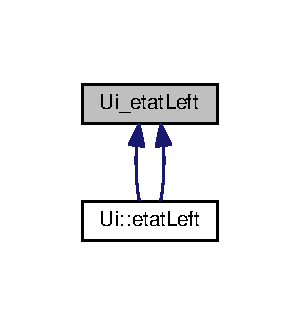
\includegraphics[width=144pt]{class_ui__etat_left__inherit__graph}
\end{center}
\end{figure}
\subsection*{Public Member Functions}
\begin{DoxyCompactItemize}
\item 
\hypertarget{class_ui__etat_left_a6ced76468569bc7b60f2f007c535091b}{void {\bfseries setup\-Ui} (Q\-Widget $\ast$\hyperlink{classetat_left}{etat\-Left})}\label{class_ui__etat_left_a6ced76468569bc7b60f2f007c535091b}

\item 
\hypertarget{class_ui__etat_left_a8a2d38afa659c1af5db423e286b41eda}{void {\bfseries retranslate\-Ui} (Q\-Widget $\ast$\hyperlink{classetat_left}{etat\-Left})}\label{class_ui__etat_left_a8a2d38afa659c1af5db423e286b41eda}

\item 
\hypertarget{class_ui__etat_left_a6ced76468569bc7b60f2f007c535091b}{void {\bfseries setup\-Ui} (Q\-Widget $\ast$\hyperlink{classetat_left}{etat\-Left})}\label{class_ui__etat_left_a6ced76468569bc7b60f2f007c535091b}

\item 
\hypertarget{class_ui__etat_left_a8a2d38afa659c1af5db423e286b41eda}{void {\bfseries retranslate\-Ui} (Q\-Widget $\ast$\hyperlink{classetat_left}{etat\-Left})}\label{class_ui__etat_left_a8a2d38afa659c1af5db423e286b41eda}

\end{DoxyCompactItemize}
\subsection*{Public Attributes}
\begin{DoxyCompactItemize}
\item 
\hypertarget{class_ui__etat_left_a274c9cd2b7f92638d78caf593154db32}{Q\-Grid\-Layout $\ast$ {\bfseries grid\-Layout}}\label{class_ui__etat_left_a274c9cd2b7f92638d78caf593154db32}

\item 
\hypertarget{class_ui__etat_left_adf0d56b2cf4c98e71862ab4e70b54745}{Q\-H\-Box\-Layout $\ast$ {\bfseries horizontal\-Layout}}\label{class_ui__etat_left_adf0d56b2cf4c98e71862ab4e70b54745}

\item 
\hypertarget{class_ui__etat_left_a0cabeb67430491c335b0a1638caa5231}{Q\-Spacer\-Item $\ast$ {\bfseries horizontal\-Spacer}}\label{class_ui__etat_left_a0cabeb67430491c335b0a1638caa5231}

\item 
\hypertarget{class_ui__etat_left_a596dbac3f6ee43e6e5ef5f469d9fd227}{Q\-Label $\ast$ {\bfseries label}}\label{class_ui__etat_left_a596dbac3f6ee43e6e5ef5f469d9fd227}

\item 
\hypertarget{class_ui__etat_left_a7122a5b8c6c69c99d33b250c507dfc50}{Q\-Spacer\-Item $\ast$ {\bfseries horizontal\-Spacer\-\_\-2}}\label{class_ui__etat_left_a7122a5b8c6c69c99d33b250c507dfc50}

\item 
\hypertarget{class_ui__etat_left_a7dc041bae70f473df0a8d2e564904191}{Q\-Push\-Button $\ast$ {\bfseries push\-Button}}\label{class_ui__etat_left_a7dc041bae70f473df0a8d2e564904191}

\item 
\hypertarget{class_ui__etat_left_a4c0c0bb1c5e29099a1154761ccb107e8}{Q\-Spacer\-Item $\ast$ {\bfseries horizontal\-Spacer\-\_\-3}}\label{class_ui__etat_left_a4c0c0bb1c5e29099a1154761ccb107e8}

\item 
\hypertarget{class_ui__etat_left_ab37a1ceedd6f15876f18720c51a3df43}{Q\-Push\-Button $\ast$ {\bfseries push\-Button\-\_\-2}}\label{class_ui__etat_left_ab37a1ceedd6f15876f18720c51a3df43}

\end{DoxyCompactItemize}


The documentation for this class was generated from the following file\-:\begin{DoxyCompactItemize}
\item 
/home/aaiiighht/\-Bureau/smartgit/bin/projet\-T\-L/automate-\/project/release/ui\-\_\-etatleft.\-h\end{DoxyCompactItemize}

\hypertarget{class_ui__etat_right}{\section{Ui\-\_\-etat\-Right Class Reference}
\label{class_ui__etat_right}\index{Ui\-\_\-etat\-Right@{Ui\-\_\-etat\-Right}}
}


Inheritance diagram for Ui\-\_\-etat\-Right\-:
\nopagebreak
\begin{figure}[H]
\begin{center}
\leavevmode
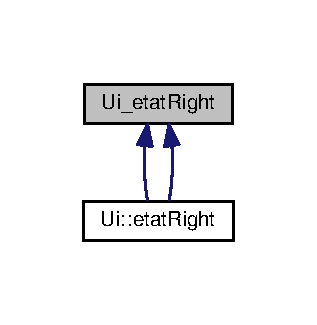
\includegraphics[width=152pt]{class_ui__etat_right__inherit__graph}
\end{center}
\end{figure}
\subsection*{Public Member Functions}
\begin{DoxyCompactItemize}
\item 
\hypertarget{class_ui__etat_right_a19c54fd43d646f353282bc374f4c1e8a}{void {\bfseries setup\-Ui} (Q\-Widget $\ast$\hyperlink{classetat_right}{etat\-Right})}\label{class_ui__etat_right_a19c54fd43d646f353282bc374f4c1e8a}

\item 
\hypertarget{class_ui__etat_right_ae20f3075c259ee0be56cd0af3111dca5}{void {\bfseries retranslate\-Ui} (Q\-Widget $\ast$\hyperlink{classetat_right}{etat\-Right})}\label{class_ui__etat_right_ae20f3075c259ee0be56cd0af3111dca5}

\item 
\hypertarget{class_ui__etat_right_a19c54fd43d646f353282bc374f4c1e8a}{void {\bfseries setup\-Ui} (Q\-Widget $\ast$\hyperlink{classetat_right}{etat\-Right})}\label{class_ui__etat_right_a19c54fd43d646f353282bc374f4c1e8a}

\item 
\hypertarget{class_ui__etat_right_ae20f3075c259ee0be56cd0af3111dca5}{void {\bfseries retranslate\-Ui} (Q\-Widget $\ast$\hyperlink{classetat_right}{etat\-Right})}\label{class_ui__etat_right_ae20f3075c259ee0be56cd0af3111dca5}

\end{DoxyCompactItemize}
\subsection*{Public Attributes}
\begin{DoxyCompactItemize}
\item 
\hypertarget{class_ui__etat_right_afb2c5e015b19f481565920291e452b91}{Q\-H\-Box\-Layout $\ast$ {\bfseries horizontal\-Layout}}\label{class_ui__etat_right_afb2c5e015b19f481565920291e452b91}

\item 
\hypertarget{class_ui__etat_right_a36783f5e7f6f101dfa06ef6ccc7384a7}{Q\-V\-Box\-Layout $\ast$ {\bfseries vertical\-Layout}}\label{class_ui__etat_right_a36783f5e7f6f101dfa06ef6ccc7384a7}

\item 
\hypertarget{class_ui__etat_right_a0519086e59266c148a10fc0276d1de61}{Q\-H\-Box\-Layout $\ast$ {\bfseries horizontal\-Layout\-\_\-3}}\label{class_ui__etat_right_a0519086e59266c148a10fc0276d1de61}

\item 
\hypertarget{class_ui__etat_right_a4b286b1151c99c60689fe086a4dbe97e}{Q\-Spacer\-Item $\ast$ {\bfseries horizontal\-Spacer}}\label{class_ui__etat_right_a4b286b1151c99c60689fe086a4dbe97e}

\item 
\hypertarget{class_ui__etat_right_a1d739dea7c4cfde35b1b6f4b8a05149c}{Q\-Label $\ast$ {\bfseries label}}\label{class_ui__etat_right_a1d739dea7c4cfde35b1b6f4b8a05149c}

\item 
\hypertarget{class_ui__etat_right_ac10b20a25fa8243c2d0188633a4cbfda}{Q\-Spacer\-Item $\ast$ {\bfseries horizontal\-Spacer\-\_\-2}}\label{class_ui__etat_right_ac10b20a25fa8243c2d0188633a4cbfda}

\item 
\hypertarget{class_ui__etat_right_acaa14fa98a4eb35e90f4d7ffcc088876}{Q\-H\-Box\-Layout $\ast$ {\bfseries horizontal\-Layout\-\_\-2}}\label{class_ui__etat_right_acaa14fa98a4eb35e90f4d7ffcc088876}

\item 
\hypertarget{class_ui__etat_right_aeb18dddd264265e8e551fcdb1957da7d}{Q\-Spacer\-Item $\ast$ {\bfseries horizontal\-Spacer\-\_\-3}}\label{class_ui__etat_right_aeb18dddd264265e8e551fcdb1957da7d}

\item 
\hypertarget{class_ui__etat_right_ac833446768b5ac7f238b3b1160c4c088}{Q\-Check\-Box $\ast$ {\bfseries check\-Box\-\_\-2}}\label{class_ui__etat_right_ac833446768b5ac7f238b3b1160c4c088}

\item 
\hypertarget{class_ui__etat_right_a2d1e013fd62a8b876b8041df17f5a8ca}{Q\-Check\-Box $\ast$ {\bfseries check\-Box}}\label{class_ui__etat_right_a2d1e013fd62a8b876b8041df17f5a8ca}

\item 
\hypertarget{class_ui__etat_right_aa961ba3779c675c3c2c6fd16ff92cf1f}{Q\-Spacer\-Item $\ast$ {\bfseries horizontal\-Spacer\-\_\-4}}\label{class_ui__etat_right_aa961ba3779c675c3c2c6fd16ff92cf1f}

\item 
\hypertarget{class_ui__etat_right_a34d98550500db0387efb8badba4f3ec1}{Q\-H\-Box\-Layout $\ast$ {\bfseries Choix}}\label{class_ui__etat_right_a34d98550500db0387efb8badba4f3ec1}

\item 
\hypertarget{class_ui__etat_right_ac5c95d3db0afea496d4fc1a49e3f4815}{Q\-Frame $\ast$ {\bfseries frame}}\label{class_ui__etat_right_ac5c95d3db0afea496d4fc1a49e3f4815}

\item 
\hypertarget{class_ui__etat_right_acda9bfa42ade85b8c556ff9d31c95e0d}{Q\-V\-Box\-Layout $\ast$ {\bfseries Show\-Choix}}\label{class_ui__etat_right_acda9bfa42ade85b8c556ff9d31c95e0d}

\end{DoxyCompactItemize}


The documentation for this class was generated from the following file\-:\begin{DoxyCompactItemize}
\item 
/home/aaiiighht/\-Bureau/smartgit/bin/projet\-T\-L/automate-\/project/release/ui\-\_\-etatright.\-h\end{DoxyCompactItemize}

\hypertarget{class_ui___main_window}{\section{Ui\-\_\-\-Main\-Window Class Reference}
\label{class_ui___main_window}\index{Ui\-\_\-\-Main\-Window@{Ui\-\_\-\-Main\-Window}}
}
Inheritance diagram for Ui\-\_\-\-Main\-Window\-:\begin{figure}[H]
\begin{center}
\leavevmode
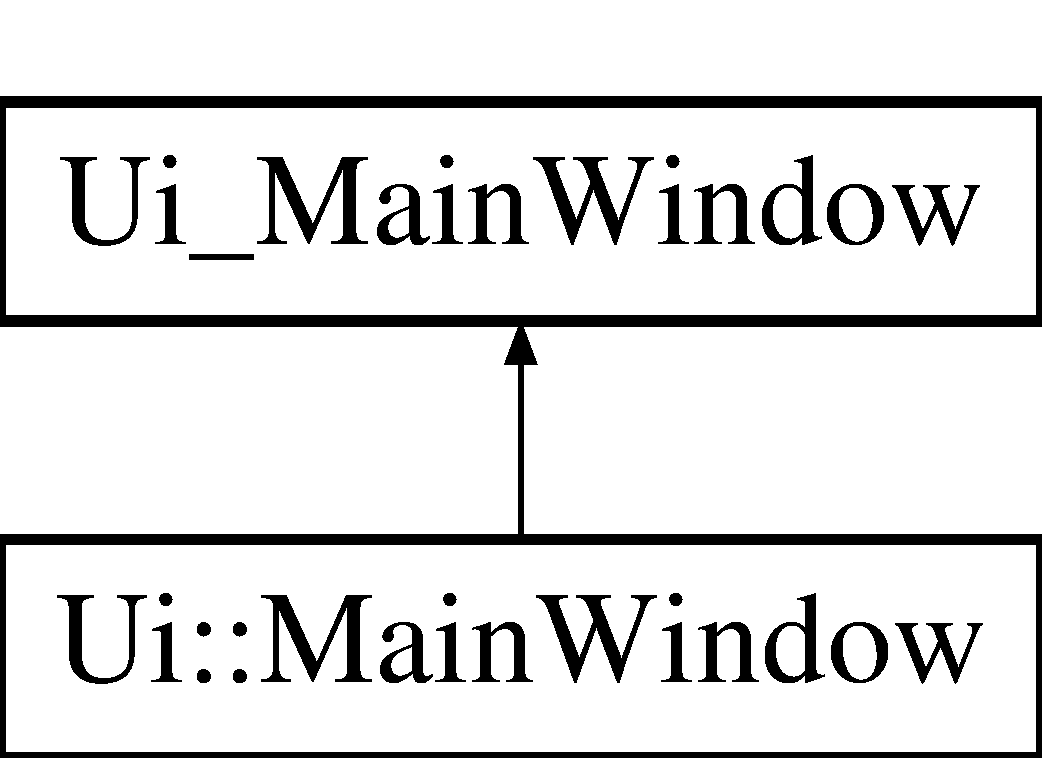
\includegraphics[height=2.000000cm]{class_ui___main_window}
\end{center}
\end{figure}
\subsection*{Public Member Functions}
\begin{DoxyCompactItemize}
\item 
\hypertarget{class_ui___main_window_acf4a0872c4c77d8f43a2ec66ed849b58}{void {\bfseries setup\-Ui} (Q\-Main\-Window $\ast$\hyperlink{class_main_window}{Main\-Window})}\label{class_ui___main_window_acf4a0872c4c77d8f43a2ec66ed849b58}

\item 
\hypertarget{class_ui___main_window_a097dd160c3534a204904cb374412c618}{void {\bfseries retranslate\-Ui} (Q\-Main\-Window $\ast$\hyperlink{class_main_window}{Main\-Window})}\label{class_ui___main_window_a097dd160c3534a204904cb374412c618}

\end{DoxyCompactItemize}
\subsection*{Public Attributes}
\begin{DoxyCompactItemize}
\item 
\hypertarget{class_ui___main_window_a20ce0f3a919249d54e02fc9ac85c9d4f}{Q\-Action $\ast$ {\bfseries action\-Fermer}}\label{class_ui___main_window_a20ce0f3a919249d54e02fc9ac85c9d4f}

\item 
\hypertarget{class_ui___main_window_a9090620adfd867b72c5f445c83b8c0ec}{Q\-Action $\ast$ {\bfseries action\-New}}\label{class_ui___main_window_a9090620adfd867b72c5f445c83b8c0ec}

\item 
\hypertarget{class_ui___main_window_a48f893f5e12be57032e2ab5b74072edb}{Q\-Action $\ast$ {\bfseries action\-Faire\-Produit}}\label{class_ui___main_window_a48f893f5e12be57032e2ab5b74072edb}

\item 
\hypertarget{class_ui___main_window_ac1f4adb06c54c11254f1a1ce0a94e037}{Q\-Action $\ast$ {\bfseries action\-Ouvrir}}\label{class_ui___main_window_ac1f4adb06c54c11254f1a1ce0a94e037}

\item 
\hypertarget{class_ui___main_window_a1b5a9f299d8a58c2f8f95ee8ddaefd2c}{Q\-Action $\ast$ {\bfseries action\-Voir}}\label{class_ui___main_window_a1b5a9f299d8a58c2f8f95ee8ddaefd2c}

\item 
\hypertarget{class_ui___main_window_a293d89eca139133a2eef134341942bd1}{Q\-Action $\ast$ {\bfseries action\-Test}}\label{class_ui___main_window_a293d89eca139133a2eef134341942bd1}

\item 
\hypertarget{class_ui___main_window_a5fbdd7ddc5864f347c0002b9990e2201}{Q\-Action $\ast$ {\bfseries action\-Clean}}\label{class_ui___main_window_a5fbdd7ddc5864f347c0002b9990e2201}

\item 
\hypertarget{class_ui___main_window_af55fe01495c55c9baf7611571c6b6158}{Q\-Action $\ast$ {\bfseries action\-Info}}\label{class_ui___main_window_af55fe01495c55c9baf7611571c6b6158}

\item 
\hypertarget{class_ui___main_window_aa3120bfbcead9ef0dda6334a525507ce}{Q\-Action $\ast$ {\bfseries action\-Determiniser}}\label{class_ui___main_window_aa3120bfbcead9ef0dda6334a525507ce}

\item 
\hypertarget{class_ui___main_window_aaa9d9c6e15ff9d685f907e3d15bcb2ee}{Q\-Action $\ast$ {\bfseries action\-Standardiser}}\label{class_ui___main_window_aaa9d9c6e15ff9d685f907e3d15bcb2ee}

\item 
\hypertarget{class_ui___main_window_a538a9134ba372db2cd40f9ccffcf4003}{Q\-Action $\ast$ {\bfseries action\-Minimiser}}\label{class_ui___main_window_a538a9134ba372db2cd40f9ccffcf4003}

\item 
\hypertarget{class_ui___main_window_a30075506c2116c3ed4ff25e07ae75f81}{Q\-Widget $\ast$ {\bfseries central\-Widget}}\label{class_ui___main_window_a30075506c2116c3ed4ff25e07ae75f81}

\item 
\hypertarget{class_ui___main_window_acd6fdc9ebacc4b25b834162380d75ce8}{Q\-H\-Box\-Layout $\ast$ {\bfseries horizontal\-Layout}}\label{class_ui___main_window_acd6fdc9ebacc4b25b834162380d75ce8}

\item 
\hypertarget{class_ui___main_window_aecd96a04789fcfec3f98d80390ad8184}{Q\-V\-Box\-Layout $\ast$ {\bfseries vertical\-Layout}}\label{class_ui___main_window_aecd96a04789fcfec3f98d80390ad8184}

\item 
\hypertarget{class_ui___main_window_a52d2f4144bb52c9b08f22917f0b523c3}{Q\-H\-Box\-Layout $\ast$ {\bfseries Top\-Layout}}\label{class_ui___main_window_a52d2f4144bb52c9b08f22917f0b523c3}

\item 
\hypertarget{class_ui___main_window_a904a0a9be0f17d57d133b6a6f8d67844}{Q\-Push\-Button $\ast$ {\bfseries bouton\-Prec}}\label{class_ui___main_window_a904a0a9be0f17d57d133b6a6f8d67844}

\item 
\hypertarget{class_ui___main_window_a582bddf7c928548f98501ac7155438d7}{Q\-Push\-Button $\ast$ {\bfseries bouton\-Suiv}}\label{class_ui___main_window_a582bddf7c928548f98501ac7155438d7}

\item 
\hypertarget{class_ui___main_window_a2b236de7a9b33cc330b47fe7177e911a}{Q\-H\-Box\-Layout $\ast$ {\bfseries Middle\-Layout}}\label{class_ui___main_window_a2b236de7a9b33cc330b47fe7177e911a}

\item 
\hypertarget{class_ui___main_window_ad32b32de02ecf0fabe0e25b8e48e034f}{Q\-Scroll\-Area $\ast$ {\bfseries scroll\-Area\-\_\-3}}\label{class_ui___main_window_ad32b32de02ecf0fabe0e25b8e48e034f}

\item 
\hypertarget{class_ui___main_window_aa2c474a2cfe4718e65713642aa1c6955}{Q\-Widget $\ast$ {\bfseries vue1}}\label{class_ui___main_window_aa2c474a2cfe4718e65713642aa1c6955}

\item 
\hypertarget{class_ui___main_window_aa5235ac9317e2feffc8a844ce126ffef}{Q\-Scroll\-Area $\ast$ {\bfseries scroll\-Area\-\_\-2}}\label{class_ui___main_window_aa5235ac9317e2feffc8a844ce126ffef}

\item 
\hypertarget{class_ui___main_window_a55ae78ec8fc0ae89aea26980898878bb}{Q\-Widget $\ast$ {\bfseries vue2}}\label{class_ui___main_window_a55ae78ec8fc0ae89aea26980898878bb}

\item 
\hypertarget{class_ui___main_window_a0cbafe1a716516744a60eb7b41120c20}{Q\-H\-Box\-Layout $\ast$ {\bfseries Lower\-Layout}}\label{class_ui___main_window_a0cbafe1a716516744a60eb7b41120c20}

\item 
\hypertarget{class_ui___main_window_ac5779d53b47a565785fec252abb1b3c6}{Q\-Scroll\-Area $\ast$ {\bfseries scroll\-Area}}\label{class_ui___main_window_ac5779d53b47a565785fec252abb1b3c6}

\item 
\hypertarget{class_ui___main_window_a2aaf3452f98efec828e1d63105a8cf0e}{Q\-Widget $\ast$ {\bfseries vue\-Tomate}}\label{class_ui___main_window_a2aaf3452f98efec828e1d63105a8cf0e}

\item 
\hypertarget{class_ui___main_window_a626cde87789b61eec68477425caf704e}{Q\-Text\-Edit $\ast$ {\bfseries label}}\label{class_ui___main_window_a626cde87789b61eec68477425caf704e}

\item 
\hypertarget{class_ui___main_window_a2be1c24ec9adfca18e1dcc951931457f}{Q\-Menu\-Bar $\ast$ {\bfseries menu\-Bar}}\label{class_ui___main_window_a2be1c24ec9adfca18e1dcc951931457f}

\item 
\hypertarget{class_ui___main_window_a7d7b4b19240d3d65b39fbfb5ee49538a}{Q\-Menu $\ast$ {\bfseries menu\-Fichier}}\label{class_ui___main_window_a7d7b4b19240d3d65b39fbfb5ee49538a}

\item 
\hypertarget{class_ui___main_window_a5fc53408d466b2c64213d2edd23bb86e}{Q\-Tool\-Bar $\ast$ {\bfseries tool\-Bar\-\_\-2}}\label{class_ui___main_window_a5fc53408d466b2c64213d2edd23bb86e}

\item 
\hypertarget{class_ui___main_window_a50fa481337604bcc8bf68de18ab16ecd}{Q\-Status\-Bar $\ast$ {\bfseries status\-Bar}}\label{class_ui___main_window_a50fa481337604bcc8bf68de18ab16ecd}

\end{DoxyCompactItemize}


The documentation for this class was generated from the following file\-:\begin{DoxyCompactItemize}
\item 
/home/aaiiighht/\-Bureau/projet\-T\-L/automate-\/project/ui\-\_\-mainwindow.\-h\end{DoxyCompactItemize}

\hypertarget{class_ui___transition}{\section{Ui\-\_\-\-Transition Class Reference}
\label{class_ui___transition}\index{Ui\-\_\-\-Transition@{Ui\-\_\-\-Transition}}
}


Inheritance diagram for Ui\-\_\-\-Transition\-:
\nopagebreak
\begin{figure}[H]
\begin{center}
\leavevmode
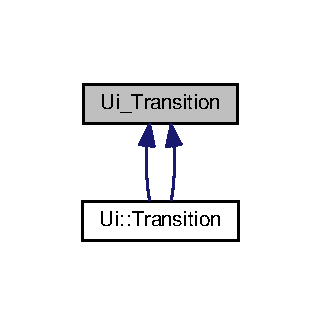
\includegraphics[width=154pt]{class_ui___transition__inherit__graph}
\end{center}
\end{figure}
\subsection*{Public Member Functions}
\begin{DoxyCompactItemize}
\item 
\hypertarget{class_ui___transition_a06f0129cc1a15bc1c50b55447578b1c5}{void {\bfseries setup\-Ui} (Q\-Widget $\ast$\hyperlink{class_transition}{Transition})}\label{class_ui___transition_a06f0129cc1a15bc1c50b55447578b1c5}

\item 
\hypertarget{class_ui___transition_ad9e6b3650adf1487f6d51e7c5d340427}{void {\bfseries retranslate\-Ui} (Q\-Widget $\ast$\hyperlink{class_transition}{Transition})}\label{class_ui___transition_ad9e6b3650adf1487f6d51e7c5d340427}

\item 
\hypertarget{class_ui___transition_a06f0129cc1a15bc1c50b55447578b1c5}{void {\bfseries setup\-Ui} (Q\-Widget $\ast$\hyperlink{class_transition}{Transition})}\label{class_ui___transition_a06f0129cc1a15bc1c50b55447578b1c5}

\item 
\hypertarget{class_ui___transition_ad9e6b3650adf1487f6d51e7c5d340427}{void {\bfseries retranslate\-Ui} (Q\-Widget $\ast$\hyperlink{class_transition}{Transition})}\label{class_ui___transition_ad9e6b3650adf1487f6d51e7c5d340427}

\end{DoxyCompactItemize}
\subsection*{Public Attributes}
\begin{DoxyCompactItemize}
\item 
\hypertarget{class_ui___transition_a1dca9708b7b32167771a6a6eb4ddd681}{Q\-H\-Box\-Layout $\ast$ {\bfseries horizontal\-Layout}}\label{class_ui___transition_a1dca9708b7b32167771a6a6eb4ddd681}

\item 
\hypertarget{class_ui___transition_a91c54b4226c964665883b2857c2e96e5}{Q\-Label $\ast$ {\bfseries label}}\label{class_ui___transition_a91c54b4226c964665883b2857c2e96e5}

\item 
\hypertarget{class_ui___transition_aa48675c679af3325e8cb26c4b6a8f3e4}{Q\-Spacer\-Item $\ast$ {\bfseries horizontal\-Spacer}}\label{class_ui___transition_aa48675c679af3325e8cb26c4b6a8f3e4}

\item 
\hypertarget{class_ui___transition_a291e72a79a44c3df5fb8c686d565fe88}{Q\-Push\-Button $\ast$ {\bfseries supress}}\label{class_ui___transition_a291e72a79a44c3df5fb8c686d565fe88}

\end{DoxyCompactItemize}


The documentation for this class was generated from the following file\-:\begin{DoxyCompactItemize}
\item 
/home/aaiiighht/\-Bureau/smartgit/bin/projet\-T\-L/automate-\/project/release/ui\-\_\-transition.\-h\end{DoxyCompactItemize}

\chapter{File Documentation}
\hypertarget{automate_8h}{\section{/home/aaiiighht/\-Bureau/projet\-T\-L/automate-\/project/automate.h File Reference}
\label{automate_8h}\index{/home/aaiiighht/\-Bureau/projet\-T\-L/automate-\/project/automate.\-h@{/home/aaiiighht/\-Bureau/projet\-T\-L/automate-\/project/automate.\-h}}
}


Représente un automate, son seul attribut est un vector d'états.  


{\ttfamily \#include $<$vector$>$}\\*
{\ttfamily \#include $<$set$>$}\\*
{\ttfamily \#include $<$list$>$}\\*
{\ttfamily \#include $<$map$>$}\\*
{\ttfamily \#include $<$string$>$}\\*
{\ttfamily \#include $<$cstdio$>$}\\*
{\ttfamily \#include $<$iostream$>$}\\*
{\ttfamily \#include $<$algorithm$>$}\\*
{\ttfamily \#include \char`\"{}etat.\-h\char`\"{}}\\*
\subsection*{Classes}
\begin{DoxyCompactItemize}
\item 
class \hyperlink{class_automate}{Automate}
\end{DoxyCompactItemize}
\subsection*{Functions}
\begin{DoxyCompactItemize}
\item 
bool \hyperlink{automate_8h_a9896d1263155efd59efe2a14ef2a807f}{equal} (list$<$ \hyperlink{classetat}{etat} $>$ \&l1, list$<$ \hyperlink{classetat}{etat} $>$ \&l2)
\begin{DoxyCompactList}\small\item\em Test l'égalité entre deux listes d'états. \end{DoxyCompactList}\item 
bool \hyperlink{automate_8h_adad60237c4515bce78983c4510406f70}{is\-Final} (list$<$ \hyperlink{classetat}{etat} $>$ l)
\begin{DoxyCompactList}\small\item\em Test si une liste d'états a au moins un état final. \end{DoxyCompactList}\end{DoxyCompactItemize}


\subsection{Detailed Description}
Représente un automate, son seul attribut est un vector d'états. 

\subsection{Function Documentation}
\hypertarget{automate_8h_a9896d1263155efd59efe2a14ef2a807f}{\index{automate.\-h@{automate.\-h}!equal@{equal}}
\index{equal@{equal}!automate.h@{automate.\-h}}
\subsubsection[{equal}]{\setlength{\rightskip}{0pt plus 5cm}bool equal (
\begin{DoxyParamCaption}
\item[{list$<$ {\bf etat} $>$ \&}]{l1, }
\item[{list$<$ {\bf etat} $>$ \&}]{l2}
\end{DoxyParamCaption}
)}}\label{automate_8h_a9896d1263155efd59efe2a14ef2a807f}


Test l'égalité entre deux listes d'états. 

Test l'égalité entre deux listes d'états l1 et l2

\begin{DoxyReturn}{Returns}
true si les listes sont égales, false sinon 
\end{DoxyReturn}
\hypertarget{automate_8h_adad60237c4515bce78983c4510406f70}{\index{automate.\-h@{automate.\-h}!is\-Final@{is\-Final}}
\index{is\-Final@{is\-Final}!automate.h@{automate.\-h}}
\subsubsection[{is\-Final}]{\setlength{\rightskip}{0pt plus 5cm}bool is\-Final (
\begin{DoxyParamCaption}
\item[{list$<$ {\bf etat} $>$}]{l}
\end{DoxyParamCaption}
)}}\label{automate_8h_adad60237c4515bce78983c4510406f70}


Test si une liste d'états a au moins un état final. 

Fonction utilisée seulement pour la déterminisation


\begin{DoxyParams}{Parameters}
{\em l} & \-: liste d'états testée\\
\hline
\end{DoxyParams}
\begin{DoxyReturn}{Returns}
true s'il y a au moins un état final dans la liste d'états, false sinon 
\end{DoxyReturn}

\hypertarget{mainwindow_8h}{\section{/home/aaiiighht/\-Bureau/projet\-T\-L/automate-\/project/mainwindow.h File Reference}
\label{mainwindow_8h}\index{/home/aaiiighht/\-Bureau/projet\-T\-L/automate-\/project/mainwindow.\-h@{/home/aaiiighht/\-Bureau/projet\-T\-L/automate-\/project/mainwindow.\-h}}
}


Représente la fenetre principale du programme. On gère ici les listeners des boutons.  


{\ttfamily \#include $<$Q\-Svg\-Widget$>$}\\*
{\ttfamily \#include $<$Q\-Main\-Window$>$}\\*
{\ttfamily \#include $<$Q\-Process$>$}\\*
{\ttfamily \#include $<$vector$>$}\\*
{\ttfamily \#include \char`\"{}automate.\-h\char`\"{}}\\*
{\ttfamily \#include $<$Q\-Push\-Button$>$}\\*
{\ttfamily \#include $<$Q\-File\-Dialog$>$}\\*
{\ttfamily \#include $<$Q\-Text\-Browser$>$}\\*
{\ttfamily \#include $<$Q\-Scroll\-Bar$>$}\\*
\subsection*{Classes}
\begin{DoxyCompactItemize}
\item 
class \hyperlink{class_main_window}{Main\-Window}
\end{DoxyCompactItemize}


\subsection{Detailed Description}
Représente la fenetre principale du programme. On gère ici les listeners des boutons. 
%--- End generated contents ---

% Index
\newpage
\phantomsection
\addcontentsline{toc}{chapter}{Index}
\printindex

\end{document}
